\chapter{Neurónové siete}

Neurónové siete sú tak úspešné pri riešení najrôznejších úloh, že sa stali synonymom 
pre celú umelú inteligenciu. V tejto časti ti poviem, ako (zjednodušene) neurónové siete fungujú
a pri tom ti navyše ukážem zopár užitočných vecí.

Neurónová sieť je program, ktorý má vstup  a výstup. Vstup aj výstup tvorí niekoľko čísel. Namiesto
za sebou napísaných príkazov, ako je to pri programoch v bežných programovacích jazykoch,
je neurónová sieť zložená zo vzájomne prepojených súčiastok, ktoré
sa volajú neuróny, lebo pripomínajú mozgové bunky.

\vskip 1ex
\centerline{
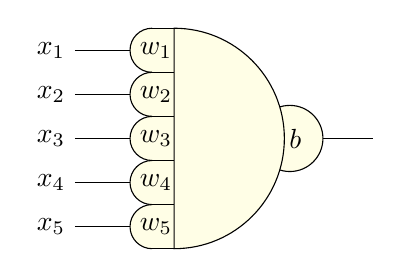
\begin{tikzpicture}
  \begin{scope}[scale=1.4]
  \draw(1.8,0)--(1,0);
  \draw[black,fill=yellow!10!white] (1.05,0) circle (0.3);
  \node at (1.1,0) {$b$};
  \def\n{5}
  \def\pos{-0.2}
  \pgfmathsetmacro{\r}{1/\n}
  \draw[draw=none,fill=yellow!10!white] (\pos,-1) rectangle (0,1);
  \foreach\i in {1,2,...,\n} {
    \pgfmathsetmacro{\y}{1-(2*\i-1)*\r}
    \draw[black,fill=yellow!10!white] (\pos,\y+\r) arc(90:270:\r);
    \draw(\pos-\r-0.5,\y) node [anchor=east] {$x_{\i}$} --(\pos-\r,\y) (\pos,\y+\r)--(0,\y+\r);
    \node[anchor=west] at (\pos-\r,\y) {$w_{\i}$};
  }
  \draw (\pos,-1) -- (0,-1);
  \draw[black, fill=yellow!10!white](0,1) arc (90:-90:1) -- cycle;
  \end{scope}
\end{tikzpicture}}

Do neurónu prichádza zvonka $n$ vstupov (čísel) $x_1,x_2,\ldots,x_n$. Neurón má pre každý vstupný 
pin určenú váhu $w_i$. Keď príde vstup, v neuróne sa spočíta súčet 
$w_1x_1+w_2x_2+\cdots+w_nx_n=\sum_{i=1}^nw_ix_i$. 
Ak  $\sum_{i=1}^nw_ix_i\ge b$, na výstupe bude 1, inak 0.

\noindent
Dajme tomu, že chceme riešiť nasledovnú (veľmi jednoduchú) úlohu: 
\cmd{Na vstupe sú 3 čísla. Zistite, či niektoré
z nich je väčšie alebo rovné ako súčet zvyšných dvoch.} Riešením môže byť
neurónová sieť, ktorá bude vyzerať takto:

\centerline{
\begin{tikzpicture}

\def\neuron(#1)#2#3#4#5#6{
  \begin{scope}[shift={(#1)}]
  \begin{scope}[scale=0.8]
    \coordinate(out#4) at (1.35,0);
  \draw[black,fill=#3!10!white] (1.05,0) circle (0.3);
    \node at (1.15,0) {{\scriptsize$#5$}};
  \def\n{3}
  \def\pos{-0.4}
  \pgfmathsetmacro{\r}{1/\n}
  \draw[draw=none,fill=#3!10!white] (\pos,-1) rectangle (0,1);
    \foreach\v/\inp[count=\i] in {#2} {
    \pgfmathsetmacro{\y}{1-(2*\i-1)*\r}
    \draw[black,fill=#3!10!white] (\pos,\y+\r) arc(90:270:\r);
    \pgfmathsetmacro{\tmp}{#6}
    \draw ([yshift=(\tmp)]\inp.east)  --(\pos-\r,\y) (\pos,\y+\r)--(0,\y+\r);
    \node[anchor=west] at (\pos-\r,\y) {{\scriptsize $\v$}};
  }
  \draw (\pos,-1) -- (0,-1);
  \draw[black, fill=#3!10!white](0,1) arc (90:-90:1) -- cycle;
  \end{scope}
  \end{scope}
}


\coordinate (inp0) at (0,0.5);
\foreach \i in {1,2,3} {
  \pgfmathtruncatemacro{\j}{\i-1}
  \node[draw=black,below=10pt of inp\j] (inp\i)  {$x_\i$};
}
  \neuron(3,1.5){1/inp1,-1/inp2,-1/inp3}{yellow}10{5}
  \neuron(3,-0.6){-1/inp1,1/inp2,-1/inp3}{green}20{0}
  \neuron(3,-2.7){-1/inp1,-1/inp2,1/inp3}{red}30{-5}

  \neuron(6,-0.6){2/out1,2/out2,2/out3}{blue}410

  \draw (out4) -- ++(0.5,0);
\end{tikzpicture}}

Žltý neurón počíta $x_1-x_2-x_3$: ak je $x_1\ge x_2+x_3$, na výstupe bude $1$, inak $0$.
Podobne zelený neurón dá na svoj výstup 1, ak $x_2\ge x_1+x_3$ a červený neurón má na výstupe 1,
ak $x_3\ge x_1+x_2$. Ak má aspoň jeden z neurónov na prvej vrstve výstup 1, na výstupe modrého
neurónu je 1, inak je tam 0.

Takýmto spôsobom sa dajú poskladať zložité siete z veľa neurónov, ktoré dokážu riešiť aj celkom 
zložité úlohy. V porovnaní s normálnymi programovacími jazykmi tu síce nemáme cykly ani podmienky,
ale na druhej strane, sieť vyrábame pre fixnú veľkosť vstupu. 
Zásadná otázka však je, prečo by sme mali produkovať programy takýmto divným spôsobom,
keď ich môžeme naprogramovať v nejakom pohodlnom programovacom jazyku.
Ide o to, že neplánujeme zostavovať neurónové siete ručne. Našim cieľom bude napísať program
(teraz myslím normálny program v C++), ktorý na vstupe dostane úlohu a vyrobí neurónovú sieť, ktorá
ju rieši. Ako môže na vstupe ``dostať úlohu'' a ako takú neurónovú sieť vyrobí, o tom budeme hovoriť o 
chvíľu. Najprv si poďme spraviť zvyčajné prípravné práce a naprogramujme si výpočet neurónovej siete.

\section*{Odbočka o  maticiach a vektoroch}
\label{mat.matice}
\def\bm#1{\ensuremath{\mathbf #1}}

Skôr, ako sa pustíme do programovania, je dobré si premyslieť, ako budeme veci označovať; pohodlné
značenie býva často polovica úspechu. Ak mám neurón s troma vstupmi $x_1, x_2, x_3$, tak vo svojom 
tele počíta $w_1x_1+w_2x_2+w_3x_3$. Ak si spomenieš na kapitolu~\ref{sect:ostrovy}, kde sme hovorili o
vektoroch, tak ak by som si predstavil, že $\vec{w} = [w_1,w_2,w_3]$  a $\vec{x} = [x_1,x_2,x_3]$
sú vektory v 3-rozmernom priestore, tak neurón počíta skalárny súčin $\vec{w}\cdot\vec{x}$.
Keby mal neurón $n$ vstupov, tiež si môžeme predstaviť, že je to vektor v nejakom priestore, až na to,
že teraz ten priestor bude $n$-rozmerný. Vôbec nevadí, že si taký priestor nevieme predstaviť,
stačí nám vedieť, že vektor v takom priestore je vyjadrený pomocou $n$ súradníc\footnote{
  Tu je vidieť, prečo sa dynamické pole v C++ volá \vb{std::vector}: je to dátová štruktúra, kde
sa dá ukladať $n$-rozmerný vektor. }a že skalárny súčin
sa počíta rovnako. Namiesto šípky hore budem vektory značiť tlstým fontom, takže
ak váhy neurónu sú $\bm{w}=[w_1,\ldots,w_n]$ a vstup je $\bm{x}=[x_1,\ldots,x_n]$, 
tak v neuróne sa počíta skalárny súčin $\bm{w}\cdot\bm{x} = \sum_{i=1}^n w_ix_i$.

Aby sa nám veci dobre rátali, tak neurónové siete, ktoré budeme vyrábať, sa budú skladať z vrstiev:
na prvej vrstve budú neuróny $N_1^{(1)}, N_2^{(1)},\ldots$, ktoré všetky budú napojené
na vstup (ale každý s inými váhami), potom na druhej vrstve budú neuróny 
$N_1^{(2)},N_2^{(2)},\ldots$, ktoré budú všetky napojené na výstupy neurónov z prvej vrstvy
atď.

\vskip 1ex
\centerline{
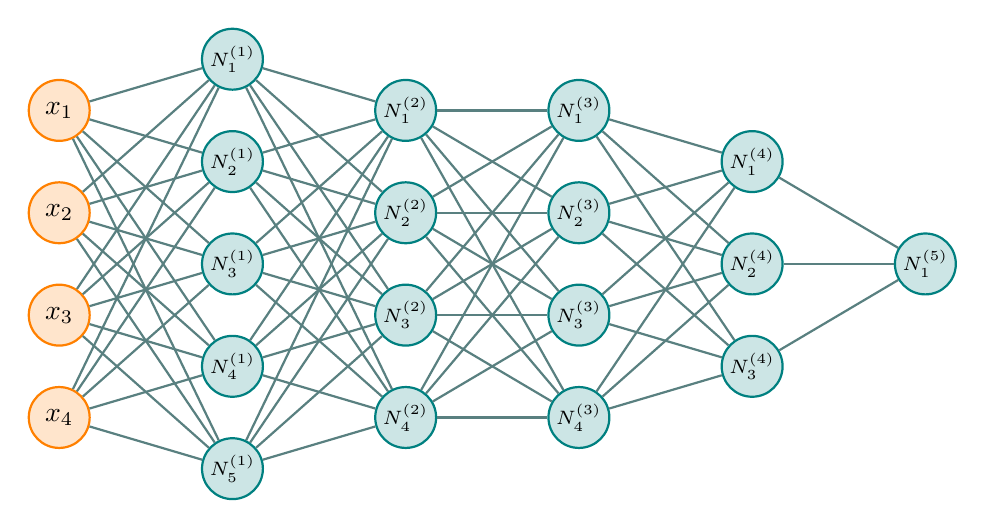
\begin{tikzpicture}[x=2.2cm,y=1.3cm,
  mynode/.style={thick,draw=\clr,fill=\clr!20,circle,inner sep=0pt, minimum size=22}]

\foreach \N [count=\lay,remember={\N as \Nprev (initially 0);}]
               in {4,5,4,4,3,1}{ % loop over layers
    \foreach \i [evaluate={\y=\N/2-\i; \x=\lay; \prev=int(\lay-1);}]
                 in {1,...,\N}{ % loop over nodes
  \ifnum\Nprev>0 
  \def\clr{teal}\def\tmp{{\scriptsize$N_\i^{(\prev)}$}}\else\def\clr{orange}\def\tmp{$x_\i$}
  \fi
      \node[mynode] (N\lay-\i) at (\x,\y) {\tmp};
      \ifnum\Nprev>0 % connect to previous layer
        \foreach \j in {1,...,\Nprev}{ % loop over nodes in previous layer
          \draw[thick,teal!30!gray] (N\prev-\j) -- (N\lay-\i);
        }
      \fi
    }
  }
\end{tikzpicture}}

Preto budeme často potrebovať vyrátať hodnotu viacerých neurónov na tom istom vstupe. Napr.
na obrázku hore je vstup $\bm{x}=[x_1,x_2,x_3,,x_4]$ a v prvej vrstve máme neuróny 
$N_1^{(1)}, N_2^{(1)},  N_3^{(1)}, N_4^{(1)}, N_5^{(1)}$. 
Váhy neurónu $N_1^{(1)}$ k vstupom $x_1,\ldots,x_4$ si označím
$\bm{w_1} = [ w_{1,1}, w_{1,2},\ldots,w_{1,4}]$, takže neurón $N_1^{(1)}$ ráta
$\sum_{i=1}^4w_{1,i}x_i=\bm{w_1}\cdot\bm{x}$.
Ak chcem vyhodnotiť všetky neuróny z prvej vrstvy, potrebujem
vyrátať skalárne súčiny \hbox{$\bm{w_1}\cdot\bm{x}$,} \hbox{$\bm{w_2}\cdot\bm{x},\ldots,\bm{w_m}\cdot\bm{x}$.}
Aby sme si skrátili zápis, vektory $\bm{w_1},\ldots,\bm{w_m}$ si napíšeme ako riadky
do tabuľky s 
$m$ riadkami a $n$ stĺpcami, pripíšeme si jeden stĺpec s vektorom \bm{x}
a výsledky sa zapíšeme do stĺpca\footnote{prečo práve do stĺpca bude zrejmé o chvíľu} takto: 
  
\def\bmatr(#1){\begin{scope}[xscale=0.9, yscale=0.7, shift={(#1)}]}
\def\ematr{\end{scope}}

\centerline{
\begin{tikzpicture}
  \def\clrs{{"sentinel","red","olive","blue","teal","orange","yellow"}}

  \bmatr(0,0)
      \node[anchor=south]  at (2,5) {$W$};
  \foreach \i in {1,...,5} {
    \pgfmathparse{\clrs[\i]}
    \xdef\tmp{\pgfmathresult}
    \node[anchor=east] at (0,5.5-\i) {\textcolor{\tmp!80!black}{$\bm{w_\i}$}};
    \filldraw[fill=\tmp!15] ($ (0,6-\i) + (0,-1) $)  rectangle +(4,1);
  }
  \draw[gray] (0,0) grid (4,5);
  \foreach \i in {1,...,5} {
    \pgfmathparse{\clrs[\i]}
    \xdef\tmp{\pgfmathresult}
    \draw[very thick, \tmp!80!black] ($ (0,6-\i) + (0,-1) $)  rectangle +(4,1);
  }
  \foreach \i in {1,...,5} {    
    \foreach \j in {1,...,4} {
      \node at ($ (\j,6-\i) + (-0.5,-0.5) $) {$w_{\i,\j}$};
    }
  }
  \node at (4.4,2.5) {$\cdot$};
  \ematr

    \bmatr(4.8,1)
      \draw[gray] (0,0) grid (1,4);
      \node[anchor=south]  at (0.5,4) {\bm{x}};
      \foreach \i in {1,...,4}
      \node at (0.5,4.5-\i) {$x_{\i}$};
      \node at (1.4,1.5) {$=$};
    \ematr
    
    \bmatr(6.6,0)
      \draw[gray] (0,0) grid (1,5);
      \node[anchor=south]  at (0.5,5) {$W\cdot\bm{x}$};
      \foreach \i in {1,...,5} {
        \pgfmathparse{\clrs[\i]}
        \xdef\tmp{\pgfmathresult}
        \node at (0.5,5.5-\i) 
        {\textcolor{\tmp!80!black}{$\bm{w_\i}\hspace*{-2pt}\cdot\hspace*{-2pt}\bm{x}$}};
      }
    \ematr


\end{tikzpicture}
}

\indexItem{Mat}{násobenie matíc}
V matematike sa tabuľka čísel volá matica ({\em matrix}). Ak teda máme maticu $W$, kde sú v riadkoch
váhy $m$ neurónov $\bm{w_1},\ldots,\bm{w_m}$ a vektor \bm{x} je vstup, obrázku
hore budeme skrátene 
hovoriť, že maticu $W$ vynásobíme vektorom \bm{x} a písať $W\cdot\bm{x}$. 
S pomocou tohoto zápisu vieme úsporne vyjadriť výpočet celej vrstvy: 
ak $i$-ty neurón porovnáva súčin $\bm{w_i}\cdot\bm{x}$ s hodnotou $b_i$,
tak rovnako dobre môžeme porovnávať $\bm{w_i}\cdot\bm{x}-b_i$ s nulou.
Preto keď si hodnoty $b_i$ zoradíme do vektora $\bm{b}=[b_1,\ldots,b_m]$,
tak výpočet celej vrstvy neurónov vieme napísať ako $W\cdot\bm{x}-\bm{b}$.

Niekedy sa nám bude hodiť aj počítať vrstvu neurónov na viacerých vstupoch naraz.
Ak ma zaujímajú vstupné vektory $\bm{x_1},\ldots,\bm{x_s}$, môžem si ich
zapísať po stĺpcoch do matice $X$ a výsledok si opäť uložiť do $s$ stĺpcov;
dostanem tak maticu rozmerov $m\times s$:

\def\bmatr(#1){\begin{scope}[xscale=1.1, yscale=0.7, shift={(#1)}]}
\def\ematr{\end{scope}}

\centerline{
\begin{tikzpicture}
  \def\clrsi{{"sentinel","red","olive","blue","teal","orange","yellow"}}
  \def\clrsii{{"sentinel","lime","violet","brown"}}

  \bmatr(0,0)
      \node[anchor=south]  at (2,5) {$W$};
  \foreach \i in {1,...,5} {
    \pgfmathparse{\clrsi[\i]}
    \xdef\tmp{\pgfmathresult}
    \node[anchor=east] at (0,5.5-\i) {\textcolor{\tmp!80!black}{$\bm{w_\i}$}};
    \filldraw[fill=\tmp!15] ($ (0,6-\i) + (0,-1) $)  rectangle +(4,1);
  }
  \draw[gray] (0,0) grid (4,5);
  \foreach \i in {1,...,5} {
    \pgfmathparse{\clrsi[\i]}
    \xdef\tmp{\pgfmathresult}
    \draw[very thick, \tmp!80!black] ($ (0,6-\i) + (0,-1) $)  rectangle +(4,1);
  }
  \foreach \i in {1,...,5} {    
    \foreach \j in {1,...,4} {
      \node at ($ (\j,6-\i) + (-0.5,-0.5) $) {$w_{\i,\j}$};
    }
  }
  \node at (4.4,2.5) {$\cdot$};
  \ematr

  \bmatr(4.8,1)
  \foreach \j in {1,...,3} {
    \pgfmathparse{\clrsii[\j]}
    \xdef\tmp{\pgfmathresult}
    \node[anchor=south] at (-0.5+\j,4) {\textcolor{\tmp!80!black}{$\bm{x_\j}$}};
    \filldraw[fill=\tmp!15] ($ (\j,0) + (-1,0) $)  rectangle +(1,4);
  }
  \draw[gray] (0,0) grid (3,4);
  \foreach \j in {1,...,3} {
    \pgfmathparse{\clrsii[\j]}
    \xdef\tmp{\pgfmathresult}
    \draw[very thick,\tmp!80!black] ($ (\j,0) + (-1,0) $)  rectangle +(1,4);
  }

  \foreach \i in {1,...,4} {    
    \foreach \j in {1,...,3} {
      \node at ($ (\j,5-\i) + (-0.5,-0.5) $) {$x_{\i,\j}$};
    }
  }
  \node at (3.4,1.5) {$=$};
  \ematr

  \bmatr(8.6,0)
  \foreach \i in {1,...,5} {    
    \foreach \j in {1,...,3} {
      \pgfmathparse{\clrsi[\i]}
      \xdef\tmp{\pgfmathresult}
      \pgfmathparse{\clrsii[\j]}
      \xdef\tmpi{\pgfmathresult}
      \filldraw[very thick, \tmpi!80!black, fill=\tmp!15] (\j-1,5-\i) rectangle +(1,1) 
      node [black,pos=0.5] {$\bm{w_\i}\bm{x_\j}$};
    }
  }
  \foreach \j in {1,...,3} {
    \node[anchor=south] at (-0.5+\j,5) {$W\bm{x_\j}$};
  }
  \draw[gray] (0,0) grid (3,5);
  \ematr


\end{tikzpicture}
}

Ak sa na tento obrázok pozrie matematik, tak vidí, že robíme presne to, čo sa v matematike deje pri násobení matíc\footnote{Spomeň si, ako sme v kapitole \ref{sect:hesovanie}
vyrábali na strane \pageref{page:nasobenie-matic} hešovaciu funkciu. Vidíš tam nejakú podobnosť?}. Ak mám maticu $A$ rozmerov $m\times n$ 
(rozmery matice budem písať ako riadky $\times$ stĺpce) a maticu $B$ rozmerov $n\times s$, tak $A\cdot B=C$ rozmerov $n\times s$ tak,
že v $i$-tom riadku a $j$-tom stĺpci matice $C$ je skalárny súčin $i$-tého riadku matice $A$ a $j$-tého stĺpca matice $B$, t,j,
$$c_{i,j}=\sum_{k=1}^na_{i,k}\cdot b_{k,j}$$

Všimni si, že nemôžeme vynásobiť hocijaké dve matice, počet stĺpcov prvej musí byť rovnaký ako počet riadkov druhej. Z toho hneď vidno, že vo všeobecnosti
$A\cdot B\not=B\cdot A$, takže treba dávať pozor na to, v akom poradí sú matice pri násobení zapísané. 
To, že sme si vektory v druhej matici písali ako stĺpce nám ale zaručí, že $A\cdot(B\cdot C)=(A\cdot B)\cdot C$ (skús si dokázať,
že to naozaj platí), takže môžeme napísať $A\cdot B\cdot C$ a nestarať sa o zátvorky.

\indexItem{Mat}{transponovaná matica}
Posledná vec v tejto odbočke je značenie $A\tran$, ktoré znamená otočenie (transpozíciu) matice $A$, t.j. výmenu riadkov a stĺpcov:
\begin{align*}
  A &= \begin{array}{|c|c|c|}\hline1&2&3\\\hline4&5&6\\\hline\end{array} & 
    A\tran &= \begin{array}{|c|c|}\hline1&4\\\hline2&5\\\hline3&6\\\hline\end{array} 
\end{align*}

\vskip 1ex
Naspäť k programovaniu. Keď si uvedomíš, že vektor je vlastne špeciálna matica, ktorá má len jeden stĺpec, na programovanie neurónových sietí nám bude
stačiť naprogramovať prácu s maticami. 

\begin{uloha}
  V kapitole~\ref{sect:cukor} sme vyrobili triedu \vb{Tabulka}. Môžeš sa ňou inšpirovať a vyrobiť triedu \vb{Matrix}, ktorá bude vedieť robiť s maticami
  čísel \prg!double!. Pridáme k nej niekoľko užitočných metód, takže by mala spĺňať takúto špecifikáciu:

\vskip 1ex
  \vbox{
  \begin{lstlisting}
using Num = double;

struct Matrix {
  int n,m;
  Num* _data;

  // konštruktory
  Matrix(int _n = 1, int _m = 1, Num init = (Num)(0));
  Matrix(int _n, int _m, const std::vector<Num>&);
  Matrix(const Matrix&);
  Matrix(Matrix&&);

  // operátory priradenia
  Matrix& operator=(const Matrix&);
  Matrix& operator=(Matrix&&);

  // prístup k dátam
  Num& operator()(int i, int j);
  const Num& operator()(int i, int j) const;

  // deštruktor
  ~Matrix();

  template <typename F> Matrix& fill(F f) { ... }
  template <typename F> Matrix& apply(F f) { ... }

  Matrix& operator+=(const Matrix& b);
  Matrix& operator-=(const Matrix& b);
  Matrix& addMultiple(Num delta, const Matrix& b);
  Matrix& addRow(const Matrix& b);    
  Matrix& addColumn(const Matrix& b); 
  Matrix transposed() const;
};
  \end{lstlisting}}

Konštruktor \prg!Matrix(Matrix&&);! je {\em move constructor}, pozri poznámku
  pre fajnšmekrov na strane \pageref{page:move-operator}. Na prístup k dátam
  treba dve funkcie, aby sme mohli mať aj konštantné aj nekonštantné premenné.
  Funkcia \vb{addMultiple} pripočíta \vb{delta}-násobok matice \vb{b}.  Funkcia
  \vb{addRow} dostane ako parameter riadok \vb{b} rozmerov $1\times m$ a
  pripočíta ho ku každému riadku matice. Podobne \vb{addColumn} so stĺpcom.
  Funkcia \vb{fill} vyplní maticu funkciou \vb{f}. Parameter \vb{f} je lambda
  (alebo funktor alebo funkcia), ktorá má dva parametre typu \vb{int} a na
  všetky prvky matice sa zavolá \prg!(*this)(i, j) = f(i, j)!. Podobne pri
  \vb{apply} má \vb{f} jeden parameter, ktorý ako vstup dostane hodnotu
  \prg!(*this)(i,j)! a modifikuje ju \prg!(*this)(i,j) = f((*this)(i,j))!.

   Okrem toho chceme samostatné funkcie

\begin{lstlisting}   
void multInto(const Matrix& a, const Matrix& b, Matrix& res); // uloží a.b do  res
Matrix operator*(const Matrix& a, const Matrix& b);
Matrix operator+(const Matrix& a, const Matrix& b);
\end{lstlisting}

\end{uloha}

Keď už máme vyriešenú prácu s maticami, môžeme začať pracovať na  neurónovej sieti. Základ bude vrstva neurónov, na začiatok urobme niečo jednoduché

\vbox{
\begin{lstlisting}
struct Layer {
  int n1;       // počet neurónov vo vrstve
  int n0;       // veľkosť predchádzajúcej vrstvy (vstupu)
  Matrix W, b;  // W: n1 x n0, kde w[i,j] = váha i-teho neurónu k j-temu vstupu
                // b: stĺpec n1 x 1
  Layer(int _n0, int _n1);       // konštruktor
  Matrix eval(const Matrix& X);  // vstup n0 x s, výstup n1 x s hodnoty neurónov
};
\end{lstlisting}
}

Vrstva bude mať \vb{n1} neurónov a bude napojená na \vb{n0} vstupných hodnôt.  Váhy neurónov budú zapamätané v matici \vb{W}. Funkcia \vb{eval} má ako parameter 
maticu, v ktorej sú v stĺpcoch uložené vstupy a vráti maticu, kde sú v stĺpcoch uložené výsledné hodnoty neurónov. Ako to čo najjednoduchšie spraviť?
Ak vyrátame $W\cdot X$, dostaneme maticu rozmerov $n_1\times s$, kde v riadku $i$ a stĺpci $j$ je $\bm{w_i}\cdot\bm{x_j}$.
Od každého stĺpca potrebujeme odrátať vektor \vb{b}, čím dostaneme pre každý neurón a každý vstup hodnotu, ktorú treba porovnať s nulou. Môžeme preto písať
(v \vb{b} chceme mať hodnoty $-b_i$ pre každý neurón)

\begin{lstlisting}
Matrix Layer::eval(const Matrix &X) {
  Matrix res = W * X;
  res.addColumn(b);
  res.apply([](double x) { return (x > 0) ? 1.0 : 0.0; });
  return res;
}
\end{lstlisting}

\indexItem{Prg}{podmienkový výraz \vb{(bool)?A:B}}
Zápis \prg!(x > 0) ? 1.0 : 0.0! som tu ešte nespomínal, ale je to skrátený zápis podmienky v jednom výraze. {\robotomono ($\clubsuit$) ? $\heartsuit$ : $\diamondsuit$ }
je výraz, ktorého hodnota je $\heartsuit$, ak $\clubsuit$ je \prg!true! a $\diamondsuit$ inak. Tu som to použil namiesto dlhšieho 
\prg!if (x > 0) return 1.0; else return 0.0;!

\begin{uloha}
  Zober si neurónovú sieť z úvodného príkladu. Napíš program, ktorý na vstupe dostane číslo $n$ a potom $n$ celých čísel. Program vyrobí neurónovú sieť
  s dvoma vrstvami (v prvej bude $n$ neurónov, v druhej jeden), ktorá zistí, či na vstupe existuje číslo, ktoré je väčšie ako súčet zvyšných. Túto sieť
  spustí na vstupných hodnotách a výsledok vypíše.
\end{uloha}

Na pohodlnejšiu prácu s jednotlivými vrstvami si ich môžeme zabaliť do jedného typu tako:

\begin{lstlisting}
struct Network {
  const unsigned long int h;  // počet vrstiev
  const vector<int> n;        // veľkosti vrstiev, n[0] je veľkosť vstupu
  vector<Layer> layers;       // vrstvy
  Network(initializer_list<int>);  // konštruktory
  Network(const vector<int>&); 
  Matrix feed(const Matrix &);
};

Network::Network(initializer_list<int> v) : h{v.size() - 1}, n{v} {
  for (int i = 0; i < h; i++) layers.emplace_back(n[i], n[i + 1]);
}

Network::Network(const vector<int>& v) : h{v.size() - 1}, n{v} {
  for (int i = 0; i < h; i++) layers.emplace_back(n[i], n[i + 1]);
}

Matrix Network::feed(const Matrix &x) {
  Matrix res(x);
  for (auto &l : layers) res = l.eval(res);
  return res;
}
\end{lstlisting}

Premenná typu \vb{Network} si pamätá počet vrstiev \vb{h}, ich veľkosti \vb{n}
a pole vrstiev \vb{layers}. Hlavná metóda je \vb{feed}, ktorá zoberie maticu
vstupných hodnôt a postupne ju ``prebuble'' cez všetky vrstvy. V tomto zápise
som použil dve nové veci, ktoré s neurónovými sieťami nesúvisia. Prvou z nich\indexItem{Prg}{trieda \vb{initializer\_list}}
je typ \vb{initializer\_list} definovaný v rovnomennej knižnici
(\prg!#include<initializer_list>!).  Nemá veľa funkcionality (v podstate má len
veľkosť \vb{size()} a iterátory \vb{begin()} a \vb{end()}), ale dá sa v
konštruktore použiť na to, aby sme premennú mohli inicializovať zoznamom
konštánt v kučeravých zátvorkách. Takže napr. volanie \vb{Newtork
net\{n,n,1\};} vyrobí sieť so vstupom veľkosti \vb{n} a dvoma vrstvami s \vb{n}
a jedným neurónom.  V konštruktore sa najprv nastaví \vb{h} (je tam
\hbox{\vb{v.size()-1}}, lebo \vb{v} obsahuje aj veľkosť vstupu) a initializer
list \vb{v} sa pošle do konštruktora vektora \vb{n}.  Druhá nová funkcia je\indexItem{Prg}{\vb{emplace\_back()}}
metóda vektora \vb{emplace\_back}. Rovnako ako \vb{push\_back} pridá prvok na
koniec vektora, ale kým \vb{push\_back} by najprv vyrobil premennú typu
\vb{Layer} a potom ju presunul do vektora, \vb{emplace\_back} dostane
parametre, ktoré sa použijú v konštruktore na vyrobenie premennej priamo na
mieste (takže je to spravidla trochu efektívnejšie). 


\vskip 2ex
Keď už vieme, ako neurónovú sieť spustiť, poďme sa pozrieť na to, ako vyrobiť
neurónovú sieť pre nejakú úlohu.  Začnime skromne. Chcem mať neurónovú sieť s
ôsmimi vstupmi, ktoré budú reprezentovať zápis 8-bitového čísla $N$ v dvojkovej
sústave. Sieť má mať jeden výstup, ktorý hovorí, či $N$ je prvočíslo.  Namiesto
toho, aby sme sieť ručne zostavovali, si iba povieme, koľko vrstiev a aké počty
neurónov v nich chceme a budeme sa snažiť napísať program, ktorý váhy neurónov doráta
tak, aby sieť čo najlepšie fungovala. 

Na to si treba v prvom rade premyslieť, ako povedať, či sieť dobre funguje. Keďže 
máme iba 256 možných vstupov, je to jednoduché: spustíme sieť na všetkých vstupoch
a spočítame, koľkokrát sa pomýlila. 

Druhá vec je, ako vyrátať váhy neurónov. Budeme to robiť podobne, ako keď sme v 
kapitole~\ref{sect:ostrovy} simulovali eróziu. Mali sme tam výškovú mapu, ktorá nám
pre bod $[x,y]$ v rovine určovala výšku terénu v tomto bode $h(x,y)$. Pre kvapku sme si pamätali
jej polohu $[x,y]$.

\vskip 2ex

\centerline{\includegraphics[width=0.7\textwidth]{asy/plocha1.pdf}}

Pohybovať sme sa vedeli v rovine, t.j. z bodu $[x,y]$ sme sa mohli pohnúť smerom $\vec\Delta=[\Delta_x,\Delta_y]$
do bodu $[x+\Delta_x,y+\Delta_y]$. Vždy sme si vybrali gradient, t.j. smer, ktorým hodnota $h(x,y)$ najviac klesá, a pohli sme sa o kúsok tým smerom.

Keby sme mali najjednoduchšiu neurónovú sieť, ktorá by mala iba jeden neurón s jedným vstupom, mohli by sme si predstaviť rovnaký obrázok. Bod $[x,y]$
v rovine by zodpovedal sieti, v ktorej je váha neurónu $x$ a porovnávacia hodnota $b$ je $y$. Výška v bode $[x,y]$ by udávala chybu siete, t.j. na koľkátich vstupoch sa
pomýli. Keď sa hýbeme bodom v rovine, hýbeme sa v priestore všetkých možných kombinácií
váh pre našu sieť.
Teraz si zober neurónovú sieť zo začiatku tejto kapitoly: má 4 neuróny a každý z nich má 4 parametre (3 vstupné váhy a hranicu $b_i$), takže dokopy viem celú sieť
opísať 16 číslami. Tie si viem prestaviť ako súradnice bodu $[x_1,x_2,\ldots,x_{16}]$ v 16-rozmernom priestore. Takýto obrázok už neviem nakresliť, ale je v podstate podobný:
namiesto dvojrozmernej roviny sa budem hýbať v 16-rozmernej, a pre každý bod mi bude moja výšková mapa udávať chybu siete. Pohnúť sa nejakým smerom znamená, že ku
každej súradnici pripočítam nejaké $\Delta_i$. 

Celý plán na nájdenie váh neurónov by vyzeral takto: začneme v nejakom náhodnom bode (t.j. so sieťou,
ktorá má náhodné váhy) a potom opakujeme cyklus: zistíme, ktorým smerom chyba siete klesá
a pohneme sa o kúsok tým smerom. Keď bude sieť dosť dobrá, tak môžeme skončiť. Ako zistiť
smer klesania chyby? Najjednoduchšie je zobrať si nejaký náhodný smer (t.j. každý parameter siete
posunúť o náhodný malý kúsok) a zistiť, ako dobrá je sieť. Ak sme sa zlepšili, tak sa tam presunieme,
ak nie, ostaneme stáť na mieste.

Toto má jeden zásadný problém: to, aká dobrá je sieť, meriame počtom vstupov, na ktorých
sa pomýli. To je celé číslo, ktoré má v našom prípade iba 256 možností. Keď sa pohnem iba o malý kúsok,
je veľká šanca, že sa počet chýb nezmení. Ak sa pohnem o veľký kus, je veľká šanca, že dolinu preskočím
a ocitnem sa na náhodnom mieste. Inými slovami, naša výšková mapa nevyzerá tak, ako na
predchádzajúcom obrázku, ale skladá sa z veľa rovných plošín. No a keď sme na takej plošine,
nevieme zistiť, ktorým smerom sa vydať.

Problém je už v samotnom neuróne, konkrétne v jeho rozhodovacej funkcii, ktorá vráti \vb{1} ak
je hodnota \hbox{$\bm{w}\cdot\bm{x}-b>0$} a \vb{0} inak. Ak váhy \bm{w} zmením iba veľmi málo, 
aj \hbox{$\bm{w}\cdot\bm{x}-b$} sa zmení len o málo, takže je len malá šanca, že sa hodnota
neurónu zmení -- sme na plošine. 
Rozhodovacia funkcia je na obrázku vľavo: pre kladné hodnoty je výsledok
$1$, pre záporné $0$. Ak by sme namiesto toho zobrali rozhodovaciu funkciu ako tá na obrázku
vpravo a neurón by rátal hodnotu 
\hbox{$\sigma(\bm{w}\cdot\bm{x}-b)$}, 
mali by sme podobnú vlastnosť: pre kladné hodnoty \hbox{$\bm{w}\cdot\bm{x}-b$}
je výsledok takmer $1$ a
pre záporné takmer $-1$. Funkcia sa navyše vždy zvažuje
smerom k nule, takže vieme, ktorým smerom 
sa treba pohnúť.


%\tikzset{external/force remake}
\begin{column}{0.5}
\begin{tikzpicture}
\begin{axis}[
    xmin=-2.5, xmax=2.5,
    ymin=-1.5, ymax=1.5,
    axis lines=center,
    axis on top=false,
    domain=-2.5:2.5,
    ylabel=$y$,
    xlabel=$x$,
    ytick={1},
    extra y ticks={-1},
    extra y tick style={yticklabel style={right, outer sep=3ex}},
    ]

    \addplot[red,very thick,smooth,domain=0:2.5] {1};
    \addplot[red,very thick,smooth,domain=-2.5:0] {0};
    \draw[black,fill=white] %(axis cs:0,0) circle(0.8mm)  
        (axis cs:0,1) circle(0.8mm);
    \draw[fill,red] (axis cs:0,0) circle(0.8mm);
    %\node [right, red] at (axis cs: 1,0.7) {$y = \mathrm{sgn}(x)$};
    
\end{axis}
\end{tikzpicture}
\end{column}
\hfill
\begin{column}{0.5}
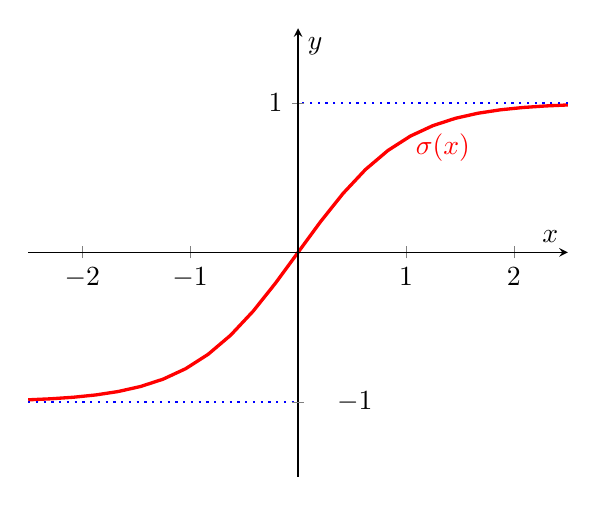
\begin{tikzpicture}
\begin{axis}[
    xmin=-2.5, xmax=2.5,
    ymin=-1.5, ymax=1.5,
    axis lines=center,
    axis on top=true,
    domain=-2.5:2.5,
    ylabel=$y$,
    xlabel=$x$,
    ytick={1},
    extra y ticks={-1},
    extra y tick style={yticklabel style={right, outer sep=3ex}},
    ]

    \addplot [mark=none,draw=red,very thick] {tanh(\x)};
    \node [right, red] at (axis cs: 1,0.7) {$\sigma(x)$};
    
    %% Add the asymptotes
    \draw [blue, dotted, thick] (axis cs:-2.5,-1)-- (axis cs:0,-1);
    \draw [blue, dotted, thick] (axis cs:+2.5,+1)-- (axis cs:0,+1);
\end{axis}
\end{tikzpicture}
\end{column}
%\tikzset{external/force remake=false}

Vpravo som použil funkciu, ktorá sa volá {\em hyperbolický tangens}\footnote{\indexItem{Mat}{funkcia tanh()}
  je to funkcia $$\mathrm{tanh}(x)=\frac{e^{2x}-1}{e^{2x}+1},$$
  kde $e\approx2.71828$ je iracionálne číslo, podobne ako $\pi$. Podobne ako $\pi$,
  aj $e$ sa prirodzene vynorí, keď začneš rátať nejaké veci, ale to teraz
  nie je dôležité. Namiesto $\mathrm{tanh}$ by sme mohli zobrať veľa 
  iných podobných funkcií, napr.{\em sigmoidu}
  $$y=\frac{1}{1+e^{-x}}$$
} a je dostupný z knižnice \vb{cmath} ako \vb{tanh(x)}. Teraz výsledok 
každého neurónu, a tým pádom aj celej siete, nebude \vb{0} alebo \vb{1}, ale
číslo z intervalu $(-1,1)$. V programe to znamená iba toľko, že funkciu 
\vb{Layer::eval} zmením takto:

\vbox{
\begin{lstlisting}
Matrix Layer::eval(const Matrix &X) {
  Matrix res = W * X;
  res.addColumn(b);
  res.apply([](double x) { return tanh(x); });
  return res;
}
\end{lstlisting}}


Výsledok celej siete budem interpretovať tak,
že záporné hodnoty beriem ako odpoveď {\em nie} a kladné ako {\em áno}.

Keď budem vyhodnocovať, ako dobrá je sieť, nebudem počítať počet vstupov, na ktorých
sa pomýli, ale budem brať do úvahy kompletné hodnoty výstupov (t.j. ako čísla z intervalu $(-1,1)$).
Pre každú hodnotu vo výslednej matici si zrátam jej chybu, t.j.
rozdiel oproti správnej odpovedi. Rozdiel ale môže byť kladný aj záporný,
čo môže robiť problémy (dve veľké chyby sa navzájom odčítajú). Preto \footnote{Sú na to aj iné, hlbšie, dôvody, ale
tie tu nepotrebujeme riešiť.} namiesto rozdielu zoberiem druhú mocninu rozdielu (je vždy kladná
a ráta sa s ňou lepšie, ako napr. s absolútnou hodnotou). Tomuto sa vraví\indexItem{Mat}{stredná kvadratická odchýlka}
{\em stredná kvadratická odchýlka} ({\em mean square error}): ak mám čísla
\hbox{$\bm{a}=[a_0,a_1,\ldots,a_{n-1}]$} a \hbox{$\bm{b}=[b_0,b_1,\ldots,b_{n-1}]$},
tak $\mathrm{mse}(\bm{a},\bm{b})=\sum_{i=0}^{n-1}(a_i-b_i)^2$.

V programe si spravím funkciu, ktorá bude porovnávať dve matice (aby výsledok nezávisel
od veľkosti matice, nakoniec ho vydelím rozmermi):

\vskip 1ex
\begin{lstlisting}
double mse(const Matrix &answer, const Matrix &truth) {
  // obe matice musia mať rovnaké rozmery
  const int n = truth.n, m = truth.m;
  double err = 0;
  for (int i = 0; i < n; i++)
    for (int j = 0; j < m; j++) {
      double tmp = truth(i, j) - answer(i, j);
      err += tmp * tmp;
    }
  err /= (double)(n * m);
  return err;
}
\end{lstlisting}

Teraz mám všetko pripravené na to, aby sme skompletizovali celý učiaci sa program.
Najprv si vyrobíme maticu \vb{data}, ktorá bude mať $8$ riadkov a $256$
stĺpcov: každý stĺpec bude mať hodnoty $-1$ a $1$ podľa toho, ako sú nastavené bity
v binárnom zápise čísla $i$. Budem mať aj maticu \vb{truth}, ktorá bude mať jeden
riadok a $256$  stĺpcov: pre každé číslo tam bude $1$ alebo $-1$ podľa toho, či je 
alebo nie je prvočíslo. Ak si napíšeš jednoduchý test \vb{prime()}, program by mohol
vyzerať napr. takto

\begin{lstlisting}
int n = 8;
Matrix data(n, 1 << n), truth(1, 1 << n);
  
for (int i = 0; i < (1 << n); i++) {
    truth(0, i) = prime(i) ? 1.0 : -1.0; 
        for (int j = 0; j < n; j++) 
            data(j, i) = (i & (1 << j) > 0) ? 1.0 : -1.0; 
}
\end{lstlisting}

Potom si vyrobím sieť s ôsmimi vstupmi. Dajme tomu, že za vstupom budem mať ešte
tri vrstvy so $16$, $8$ a jedným neurónom (to bude výstup). Keďže budem potrebovať
k sieti pridávať náhodný šum a potom ho možno zobrať naspäť, najjednoduchšie je
k triede \vb{Network} pridať metódu \vb{addNoise}, ktorá na vstupe dostane okrem
iného seed pre náhodný generátor; takto viem ľahko urobiť tú istú postupnosť náhodných čísel
(stačí poslať rovnaký seed). Spravil som to takto:


\begin{lstlisting}
void Network::addNoise(unsigned int seed, int sgn, double val) {
  mt19937 rnd;
  uniform_real_distribution<> dis(-val, val);
  rnd.seed(seed);
  for (auto &l : layers)
    for (auto m : {&l.W, &l.b})
      m->apply([&](double x) { return x + sgn * dis(rnd); });
}
\end{lstlisting}

Na začiatku nastavím sieť na náhodný bod:

\begin{lstlisting}
  Network net{n, 16, 8, 1};
  net.addNoise(random_device{}(), 1, 0.01);
\end{lstlisting}

V hlavnom cykle si vyrobím náhodné číslo. To použijem ako seed, s pomocou
ktorého pridám do siete náhodný šum. Vypočítam si odpoveď siete na všetkých vstupoch
a zrátam si chybu. Ak je väčšia ako doterajšia, odrátam od siete ten istý šum
(použijem rovnaký seed, ale opačné znamienko).

\vskip 1ex
\begin{lstlisting}
mt19937 rnd(random_device{}());
double last_err = 1e50;
Matrix answer;
int cnt = 0;
do {
  auto seed = rnd();
  net.addNoise(seed);
  answer = net.feed(data);
  auto err = mse(answer, truth);
  if (err < last_err)
    last_err = err;
  else
    net.addNoise(seed, -1);
  cout << cnt++ << " " << last_err << endl;
} while (last_err > 5e-3);
\end{lstlisting}

Keď som to dal celé dokopy a vyskúšal, typicky som dostal niečo takéto:

\vskip 1ex
%\tikzset{external/force remake}
\begin{tikzpicture}
  \def\plota[#1]#2#3{%
    \addplot[#1,mark=*, 
    line join=round, mark size=0pt] table [y=#2, x=t]{data/learn_primes_1.out};
    \addlegendentry{\vb{#3}}
  }
\begin{axis}[
  width=\textwidth, 
  height=8cm,
  xlabel=počet opakovaní cyklu,
  ylabel={},
  legend cell align={left},
  legend pos = north west,
  %ymax=0.9,
  scaled x ticks=false,
  %scaled y ticks=false,
  legend style={at={(0,0)},anchor=south west, outer sep = 2ex},
    /pgf/number format/.cd,
        1000 sep={}
]
  \plota[blue!80]{err}{chyba siete}
  \plota[orange!80]{good}{percento správnych výsledkov}
\end{axis}
\end{tikzpicture}
%\tikzset{external/force remake=false}

Vidno, že chyba siete postupne klesá, ale treba na to pomerne veľa iterácií: v mojom prípade
zrhuba $80 000$, kým sa sieť naučila všetky čísla správne. Zároveň vidno, že prvočísel je pomerne
málo, takže mať $80\%$ úspešnosť dokáže aj úplne hlúpa sieť.

\begin{uloha}
  Vyskúšaj si, ako sa zmení trénovanie, keď meníš veľkosť siete. Čo sa stane, ak
  je primalá? A čo ak je priveľká?
\end{uloha}

Toto bola, samozrejme, trochu hračkárska úloha, keďže sme sa starali iba o 256 rôznych vstupov. 
Chcelo by to skúsoť si väčšie siete, ale náš spôsob učenia, keď si vždy vyberáme náhodný smer, je veľmi pomalý.
Preto skôr, ako pokročíme smerom k zaujímavejším úlohám, najprv vymyslíme spôsob, ako siete
trénovať rýchlejšie. Konkrétne budeme chcieť zrátať smer, ktorým výšková mapa klesá 
(a teda ktorým sa máme posunúť). Na to ale potrebujeme ešte jednu matematickú odbočku.


\section*{Matematická odbočka: o deriváciách}
\label{mat.derivacie}

Predstav si, že si nakreslím graf nejakej funkcie $y=f(x)$. Keď si zoberiem  nejaké číslo
$x_0$, bod $P=[x_0,f(x_0)]$ leží na grafe funkcie. Teraz ma zaujíma dotyčnica\footnote{t.j. priamka, ktorá má s grafom spoločný iba jeden bod} ku grafu v bode $P$.
Konkrétne, chcem vedieť, aký uhol $\alpha$ zviera dotyčnica s osou $x$. Keby som ho poznal, tak viem, že ak sa na osi $x$ pohnem o nejaký hocijaký kúsok $\Delta$, 
tak priamka stúpne o $\Delta\cdot\tan(\alpha)$. \indexItem{Mat}{tangens}To $\tan(\alpha)$ je nejaké číslo\footnote{Volá sa {\em tangens} a patrí medzi goniometrické funkcie, podobne ako $\sin$
a $\cos$ z kapitoly~\ref{sect:sin_cos}. Tangens je pomer protiľahlej a priľahlej strany pravouhlého trojuholníka, inými slovami $\tan(\alpha)=\frac{\sin(\alpha)}{\cos{\alpha}}$.}, 
ktoré závisí iba od uhla $\alpha$ (lebo pre vešetky voľby $\Delta$ sú tyrkysové trojuholníky z ľavého obrázka podobné). Dotyčnica sa v domácnosti hodí: keby som pozeral iba veľmi blízko 
$x_0$, mohol by som sa tváriť, že namiesto (možno zložitej) funkcie $f(x)$ mám jednoduchú priamku.


\vskip 1ex
\centerline{
  \includegraphics{asy/deriv1.pdf}
\hfill
\includegraphics{asy/deriv2.pdf}
}

Ak neviem zrátať priamo dotyčnicu, môžem si skúsiť zrátať niečo, 
čo sa jej dosť podobá. Zoberiem si malý kúsok $\Delta$ a spravím si 
zelenú priamku z pravého obrázka, ktorá
prechádza bodom $P$ a bodom $[x_0+\Delta, f(x_0+\Delta)]$. O tjeto priamke ľahko zistím tangens jej uhla: je to $\frac{f(x_0+\Delta)-f(x_0)}{\Delta}$. Čím menšie $\Delta$ si zvolím,
tým bude výsledná priamka vernejšie reprezentovať dotyčnicu. 

Poďme si to skúsiť zrátať napr. pre funkciu $f(x)=x^2$. Pre zvolené $\Delta$ bude $\tan(\alpha)$
$$\tan(\alpha)=\frac{(x_0+\Delta)^2-x_0^2}{\Delta}.$$
Ak sa bude $\Delta$ blížiť k nule, budem v čitateli aj menovateli dostávať menšie a menšie čísla a o výsledku neviem povedať nič. Napíšem si to isté inak:
$$\tan(\alpha)=\frac{(x_0+\Delta)^2-x_0^2}{\Delta}=\frac{x_0^2+2x_0\Delta+\Delta^2-x_0^2}{\Delta}=2x_0+\Delta.$$
Teraz je jasné, že  čím bližšie bude $\Delta$ k nule, tým bližšie bude $\tan(\alpha)$ k $2x_0$. Môžem teda celkom pokojne povedať, že dotyčnica k $x^2$ v bode $x_0$ má sklon
$2x_0$.\indexItem{Mat}{derivácia} Sklon dotyčnice v nejakom bode sa volá {\em derivácia}, takže sme práve zrátali, že 
derivácia funkcie $x^2$ v bode $x_0$ je $2x_0$. Na deriváciu sa môžem pozrieť ako na funkciu,
ktorá pre dané $x$ vráti deriváciu v bode $x$:
ak mám pôvodnú funkciu $f(x)=x^2$, tak jej derivácia je funkcia $2x$. Označovať sa zvykne rôzne. 
Lagrange deriváciu označoval čiarkou, napr. ak $f(x)=x^2$, tak $f'(x)=2x$.
Keď napr. chceme zdôrazniť, podľa akej premennej derivujeme, môžeme písať aj
$\odv{x^2}{x}=2x$. V každom prípade, derivácia nám hovorí, ako rýchlo v danom 
bode $x_0$ funkcia rastie: ak sa pohneme o malý kúsok $\Delta$, funkcia narastie\footnote{
Ak je derivácia kladná, funkcia rastie, ak je záporná, tak funkcia klesá. Ak je nulová, tak
nerastie ani neklesá. 
\IGNORE{
To znamená, že ak funkcia má niekde maximum alebo minimum (napr.
funkcia $x^2$ má minimum v bode $0$), má tam nulovú deriváciu. Pomocou toho sa dajú hľadať maximá a minimá
rôznych funkcií.}}
zhruba o 
$\Delta\cdot f'(x_0)$. 

\indexItem{Mat}{derivácia mocniny, súčtu a súčinu}
Poďme si zopár derivácií zrátať. Vieme spraviť $x^2$, tak skúsme $f(x)=x^a$ pre nejaké celé číslo $a>2$. Roznásobme si zátvorky v 
$(x_0+\Delta)^a$. Napr. pre $a=3$ to bude vyzerať
\def\ox{\textcolor{orange}{x_0}}
\def\od{\textcolor{orange}{\Delta}}
\def\tx{\textcolor{teal}{x_0}}
\def\td{\textcolor{teal}{\Delta}}
\def\mx{\textcolor{magenta}{x_0}}
\def\md{\textcolor{magenta}{\Delta}}
\def\oxd{\textcolor{orange}{(x_0+\Delta)}}
\def\txd{\textcolor{teal}{(x_0+\Delta)}}
\def\mxd{\textcolor{magenta}{(x_0+\Delta)}}
\begin{align*}
  (x_0+\Delta)^3&=\oxd\txd\mxd=\\
  &= \ox\txd\mxd + \od\txd\mxd=\\
  &=\ox\tx\mxd+\ox\td\mxd +\od\tx\mxd + \od\td\mxd =\\
  &=\ox\tx\mx+\ox\tx\md+\ox\td\mx+\ox\td\md+\od\tx\mx+\od\tx\md+\od\td\mx+\od\td\md
\end{align*}

Z tohoto by malo byť jasné, že ak roznásobím $(x_0+\Delta)^a$, dostanem súčet $2^a$ sčítancov tak, že z každej zátvorky si vyberiem buď $x_0$ alebo $\Delta$. Takže budem
mať jeden sčítanec $x_0^a$, $a$ sčítancov $\Delta\cdot x_0^{a-1}$ a všetky ostatné budú obsahovať člen $\Delta^2$. Preto $(x_0+\Delta)^a=x_0^a+a\Delta x_0^{a-1}+\Delta^2\heartsuit$,
kde $\heartsuit$ je niečo zložené z $x_0$ a $\Delta$, čo ma teraz príliš nezaujíma. Idem rátať sklon priamok podobne ako pred chvíľou:

$$\tan(\alpha)=\frac{(x_0+\Delta)^a-x_0^a}{\Delta}=\frac{x_0^a+a\Delta x_0^{a-1}+\Delta^2\heartsuit-x_0^a}{\Delta}=\frac{a\Delta x_0^{a-1}+\Delta^2\heartsuit}{\Delta}
=ax_0^{a-1}+\Delta\heartsuit$$

Keď beriem menšie a menšie $\Delta$, $\Delta\heartsuit$ bude viac a viac bližšie k nule. Preto 
$\left(x^a\right)'=ax^{a-1}$. Platí to aj pre iné hodnoty $a$? Ak $a=0$, $x^0=1$ a uhol je zjavne $0$. Fajn. Čo tak $a=-1$?
Vtedy mám\footnote{pripomeň si poznámku pod čiarou na str. \pageref{page:umocnovanie}} 
$x^{-1}=\frac{1}{x}$, takže si zrátam:

$$\tan(\alpha)=\frac{\frac{1}{x_0+\Delta}-\frac{1}{x_0}}{\Delta}
=\frac{\frac{x_0-(x_0+\Delta)}{x_0(x_0+\Delta)}}{\Delta}
=\frac{x_0-(x_0+\Delta)}{x_0(x_0+\Delta)\Delta}=-\frac{1}{x_0(x_0+\Delta)}
$$

takže keď je $\Delta$ veľmi blizko nuly, je $\tan(\alpha)$ blízko $-\frac{1}{x_0^2}$, takže 
$\left(x^{-1}\right)'=-\frac{1}{x^2}=-1\cdot x^{-2}$. Skvelé. A čo ak $a=\frac{1}{2}$?
Vtedy $x^\frac{1}{2}=\sqrt{x}$, takže mám

$$\tan(\alpha)=\frac{\sqrt{x_0+\Delta}-\sqrt{x_0}}{\Delta} = \frac{\sqrt{x_0+\Delta}-\sqrt{x_0}}{\Delta}
\textcolor{magenta}{\cdot\frac{\sqrt{x_0+\Delta}+\sqrt{x_0}}{\sqrt{x_0+\Delta}+\sqrt{x_0}}}=
\frac{x_0+\Delta-x_0}{\Delta\left(\sqrt{x_0+\Delta}+\sqrt{x_0}\right)}=
\frac{1}{\sqrt{x_0+\Delta}+\sqrt{x_0}}
$$

a teda keď je $\Delta$ menšie a menšie dostávam 
$\left(\sqrt{x}\right)'=\frac{1}{2\sqrt{x}}=\frac{1}{2}x^{-\frac{1}{2}}$. 
S trochou námahy by sa dalo vidieť, že vzťah $\left(x^a\right)'=ax^{a-1}$
platí pre hocijaké $a$. To sa nám ešte bude hodiť.

Ešte sa chvíľu s deriváciami hrajme: ak mám funkcie $f(x)$ a $g(x)$ a spravím si funkciu $h(x)=f(x)+g(x)$. Viem zistiť $h'(x)$? Napíšem si ako vždy:

$$\tan(\alpha)=\frac{\left(f(x_0+\Delta)+g(x_0+\Delta)\right)-\left(f(x_0)+g(x_0)\right)}{\Delta}=\frac{f(x_0+\Delta)-f(x_0)}{\Delta}+\frac{g(x_0+\Delta)-g(x_0)}{\Delta}$$

Preto vidím, že $h'(x)=f'(x)+g'(x)$. Podobne sa dá vidieť, že ak mám funkciu $f(x)$ a spravím si 
\hbox{$g(x)=c\cdot f(x)$,} tak $g'(x)=c\cdot f'(x)$. S násobením je to trošku 
zložitejšie. Ak mám funkcie $f(x)$ a $g(x)$ a urobím si $h(x)=f(x)\cdot g(x)$, tak dostávam

$$\tan(\alpha)=\frac{\left(f(x_0+\Delta)g(x_0+\Delta)\right)-\left(f(x_0)g(x_0)\right)}{\Delta}
$$

Čo s tým? Spravím fintu, že do čitateľa si pridám rafinovane napísanú nulu

\begin{align*}
  \tan(\alpha)&=\frac{f(x_0+\Delta)g(x_0+\Delta)-f(x_0)g(x_0)+\textcolor{magenta}{f(x_0+\Delta)g(x_0)-f(x_0+\Delta)g(x_0) }}{\Delta}=\\
  &=f(x_0+\Delta)\left(\frac{g(x_0+\Delta)-g(x_0)}{\Delta}\right)+g(x_0)\left(\frac{f(x_0+\Delta)-f(x_0)}{\Delta}\right)
\end{align*}

Keď je $\Delta$ strašne maličké, tak $f(x_0+\Delta)$ je čoraz bližšie k $f(x_0)$ a tie veľké zátvorky sa blížia k dotyčniciam pre $g(x_0)$ a $f(x_0)$. Preto vidím, že
$h'(x)=f(x)g'(x)+f'(x)g(x)$.

Na lepšiu ilustráciu si zoberme funkciu $f(x)= 8x^3-3x^4+18x^2$ (na obrázku oranžová) a pýtajme sa,
akú najväčšiu hodnotu môže nadobudnúť. Vieme si ľahko zrátať jej deriváciu: najprv ju rozdelíme na
súčet troch členov, z ktorých každý má tvar $cx^a$ a tie už zderivovať vieme. Takže dostaneme,
že $f'(x)=24x^2-12x^3+36x$ (na obrázku modrá funkcia).

\centerline{\includegraphics{asy/deriv3.pdf}}

Ak má mať $f(x)$ v nejakom bode $x_0$ maximum, tak v $x_0$ nesmie rásť, a teda $f'(x_0)=0$.
Takže stačí zistiť, kde všade je $f'(x)=0$ a v jednom z tých bodov bude maximum. Napíšem si
$f'(x)$ v tvare \hbox{$f'(x)=-12x(x^2-2x-3)=-4x(x+1)(x-3)$,} z ktorého vidno, že $f'(x)=0$ v bodoch
$-1$, $0$ a $3$. A je to.

\indexItem{Mat}{derivácia zloženej funkcie}
Ešte jedna vec sa bude hodiť pre počítanie s deriváciami, a to derivácia zloženej funkcie. 
Zoberme si kružnicu so stredom v bode $[0,0]$ a polomerom $1$ a poďme k nej spraviť dotyčnicu v 
nejakom bode $P$. Narysoval by som to ľahko: urobím polpriamku $\overrightarrow{0P}$ a
na ňu kolmicu v bode $P$.
Ako to ale zrátať? Kružnicu tvoria body so vzdialenosťou $1$ od stredu, preto pre ne platí
$x^2+y^2=1^2$. Keď si z toho vyjadrím $y$, dostanem, že kružnica (presnejšie jej horná
polovica) je grafom funkcie $h(x)=\sqrt{1-x^2}$. Vektor $\vec{v}=[1,h'(x_0)]$ mi preto dáva 
dotyčnicu, ktorú chcem. 
Keď zrátam $h'(x_0)$, budem môcť overiť, že vektor $\vec{v}$ je kolmý na $\overrightarrow{0P}$.

\vskip 1ex
\centerline{\includegraphics{asy/deriv_kruh.pdf}}

Ako zrátam deriváciu $\sqrt{1-x^2}$? Tá funkcia síce vyzerá hrozivo, ale 
keď sa lepšie prizriem, vidím, že je zložená z dvoch funkcií,
ktoré už derivovať viem. Keď označím $g(x)=1-x^2$ a $f(x)=\sqrt{x}$, tak
$\sqrt{1-x^2}=f(g(x))$ (t.j. najprv sa zráta $g(x)$ a výsledok sa použije ako vstup do 
funkcie $f(\cdot)$).

Poďme sa teda pozrieť zbližšia na deriváciu $f(g(x))$. 

$$\tan(\alpha)=\frac{f(g(x_0+\Delta))-f(g(x_0))}{\Delta}
\textcolor{magenta}{\cdot\frac{g(x_0+\Delta)-g(x_0)}{g(x_0+\Delta)-g(x_0)}}
=
\frac{f(g(x_0+\Delta))-f(g(x_0))}{\textcolor{magenta}{g(x_0+\Delta)-g(x_0)}}
\cdot\frac{\textcolor{magenta}{g(x_0+\Delta)-g(x_0)}}{\Delta}
$$

V prvom kroku som si napísal rafinovanú jednotku. To môžem urobiť, len ak 
$g(x_0+\Delta)\not=g(x_0)$; v opačnom prípade by bolo treba trochu inú úvahu 
(ale dopadlo by to rovnako). V tom, čo som dostal, je 
$\frac{g(x_0-\Delta)-g(x_0)}{\Delta}$
pre veľmi malé $\Delta$ v podstate $g'(x_0)$. Čo sa dá pre malé $\Delta$ povedať o 
$$\frac{f(g(x_0+\Delta))-f(g(x_0))}{\textcolor{orange}{g(x_0+\Delta)}-g(x_0)}?$$
Hodnota $\textcolor{orange}{g(x_0+\Delta)}$ je približne $\textcolor{orange}{g(x_0)+\Delta g'(x_0)}$. 
Keďže $g'(x_0)$ je nejaké konkrétne číslo, keď zmenšujem $\Delta$ na veľmi malé, je aj $\Delta\cdot g'(x_0)$ veľmi malé.
Keď si označím $y_0=g(x_0)$ a $\Delta'=\Delta g'(x_0)$,
budem mať
$$\left(f(g(x_0))\right)'=\frac{f(\Delta'+y_0)-f(y_0)}{\Delta'}\cdot g'(x_0)$$
a teda vidím, že $(f(g(x)))'=f'(g(x))g'(x)$. Tento vzťah je možno zrozumiteľnejší,
keď ho zapíšem takto:
$$\odv{h}{x}=\odv{h}{g}\cdot\odv{g}{x}$$

To znamená, že keď mám nejakú funkciu  $h$ (napr. $h=\sqrt{1-x^2}$), 
označím si nejakú časť ako $g$ (napr.
$g(x)=1-x^2$). Teraz sa na $g$ môžem pozrieť ako na novú premennú, takže $h$ závisí od $g$ a $g$ závisí od $x$. 
Preto keď trochu zmením $x$, $g$ sa zmení o $\odv{g}{x}$
(a.k.a. $g'(x)$) a zaujíma ma, ako sa zmení $h(g)$.

V našom príklade $g(x)=1-x^2$, preto $\odv{g}{x}=g'(x)=-2x$. Vonkajšia funkcia 
$f(g(x)) = h(g) = \sqrt{g}$, preto $\odv{h}{g}=\frac{1}{2}g^{-\frac{1}{2}}$. Preto 
$$\odv{\sqrt{1-x^2}}{x}=\odv{\sqrt{g}}{g}\cdot\odv{(1-x^2)}{x}=\frac{1}{2}g^{-\frac{1}{2}}\cdot(-2x)
=\frac{1}{2(1-x)^\frac{1}{2}}\cdot(-2x)=\frac{-x}{\sqrt{1-x^2}} 
$$

Teraz si môžem overiť, že vektor $\vec{v}=\left[1,-\frac{x_0}{\sqrt{1-x_0^2}}\right]$ je kolmý na 
$\overrightarrow{0P}=\left[x_0,\sqrt{1-x_0^2}\right]$.
Na to sa hodí, čo sme si hovorili o skalárnom súčine na str.~\pageref{page:dotproduct-angle}: vyrátam si
$$\vec{u}\cdot\overrightarrow{0P}=x_0-\frac{x_0}{\sqrt{1-x_0^2}}\cdot\sqrt{1-x_0^2}=x_0-x_0=0$$
preto vidím, že keď skalárny súčin je $0$, kosínus uhla medzi vektormi musí byť $0$, a teda $\overrightarrow{0P}$ a $\vec{v}$ sú
na seba kolmé.


Zhrňme si, čo vieme o deriváciách:

\vskip 1ex
\centerline{\fcolorbox{magenta}{magenta!3!white}{\parbox{0.9\textwidth}{%
\begin{enumerate}
    \item $\left(x^a\right)'=ax^{a-1}$
    \item $\left(c\cdot f(x)\right)'=c\cdot f'(x)$
    \item $\left(f(x)+g(x)\right)'=f(x)'+g'(x)$
    \item $\left(f(x)\cdot g(x)\right)'=f'(x)g(x)+f(x)g'(x)$
    \item $\left(f(g(x))\right)'=f'(g(x))\cdot g'(x)$
\end{enumerate}
  \vspace*{-1ex}
}}}


Aby som sa príliš nerozkokošil s deriváciami, treba si pripomenúť, načo to celé rozprávam: hľadáme spôsob, ako upraviť parametre siete tak, aby chyba čo najviac klesla.
Zoberme si opäť najjednoduchšiu možnú sieť s jediným neurónom, ktorý má parametre $w$, $b$ a pre vstup $x$ vyráta $\tanh(xw+b)$. Dajme tomu, že chceme riešiť úlohu s jediným vstupom
$x_1$, ktorého správny výstup je $y_1$. Odpoveď siete na vstupe $x_1$ je $\tanh(wx_1+b)$, chyba siete (stredná kvadratická odchýlka) je funkcia parametrov $w$ a $b$:
$\mathrm{err}(w,b)=\left(\tanh(wx_1+b)-y_1\right)^2$. Ak mám ``sieť'' s parametrami $w$, $b$, chcem zistiť, ktorým smerom sa pohnúť, aby sa chyba zmenšila. Na to nám
poslúži {\em gradient} funkcie\footnote{Už sme ho spomenuli, v časti o 
erózii na str, \pageref{page:gradient}, ale vtedy nám stačila iba zjednodušená predstava. Teraz to budeme
potrebovať spraviť poriadnejšie.}.

\indexItem{Mat}{gradient funkcie viacerých premenných}
Mám nejakú funkciu dvoch premenných $f(x,y)$ a bod $p=[p_x,p_y]$.
Keď si zafixujem hodnotu $y=p_y$ a dosadím do $f(x,y)$,
dostanem funkciu jednej premennej $f_{y=p_y}(x)$. Body, v ktorých je $y=p_y$ tvoria v 3D rovinu.
Funkcia $f_{y=p_y}(x)$ je prienik 3D výskovej mapy s touto rovinou:

\centerline{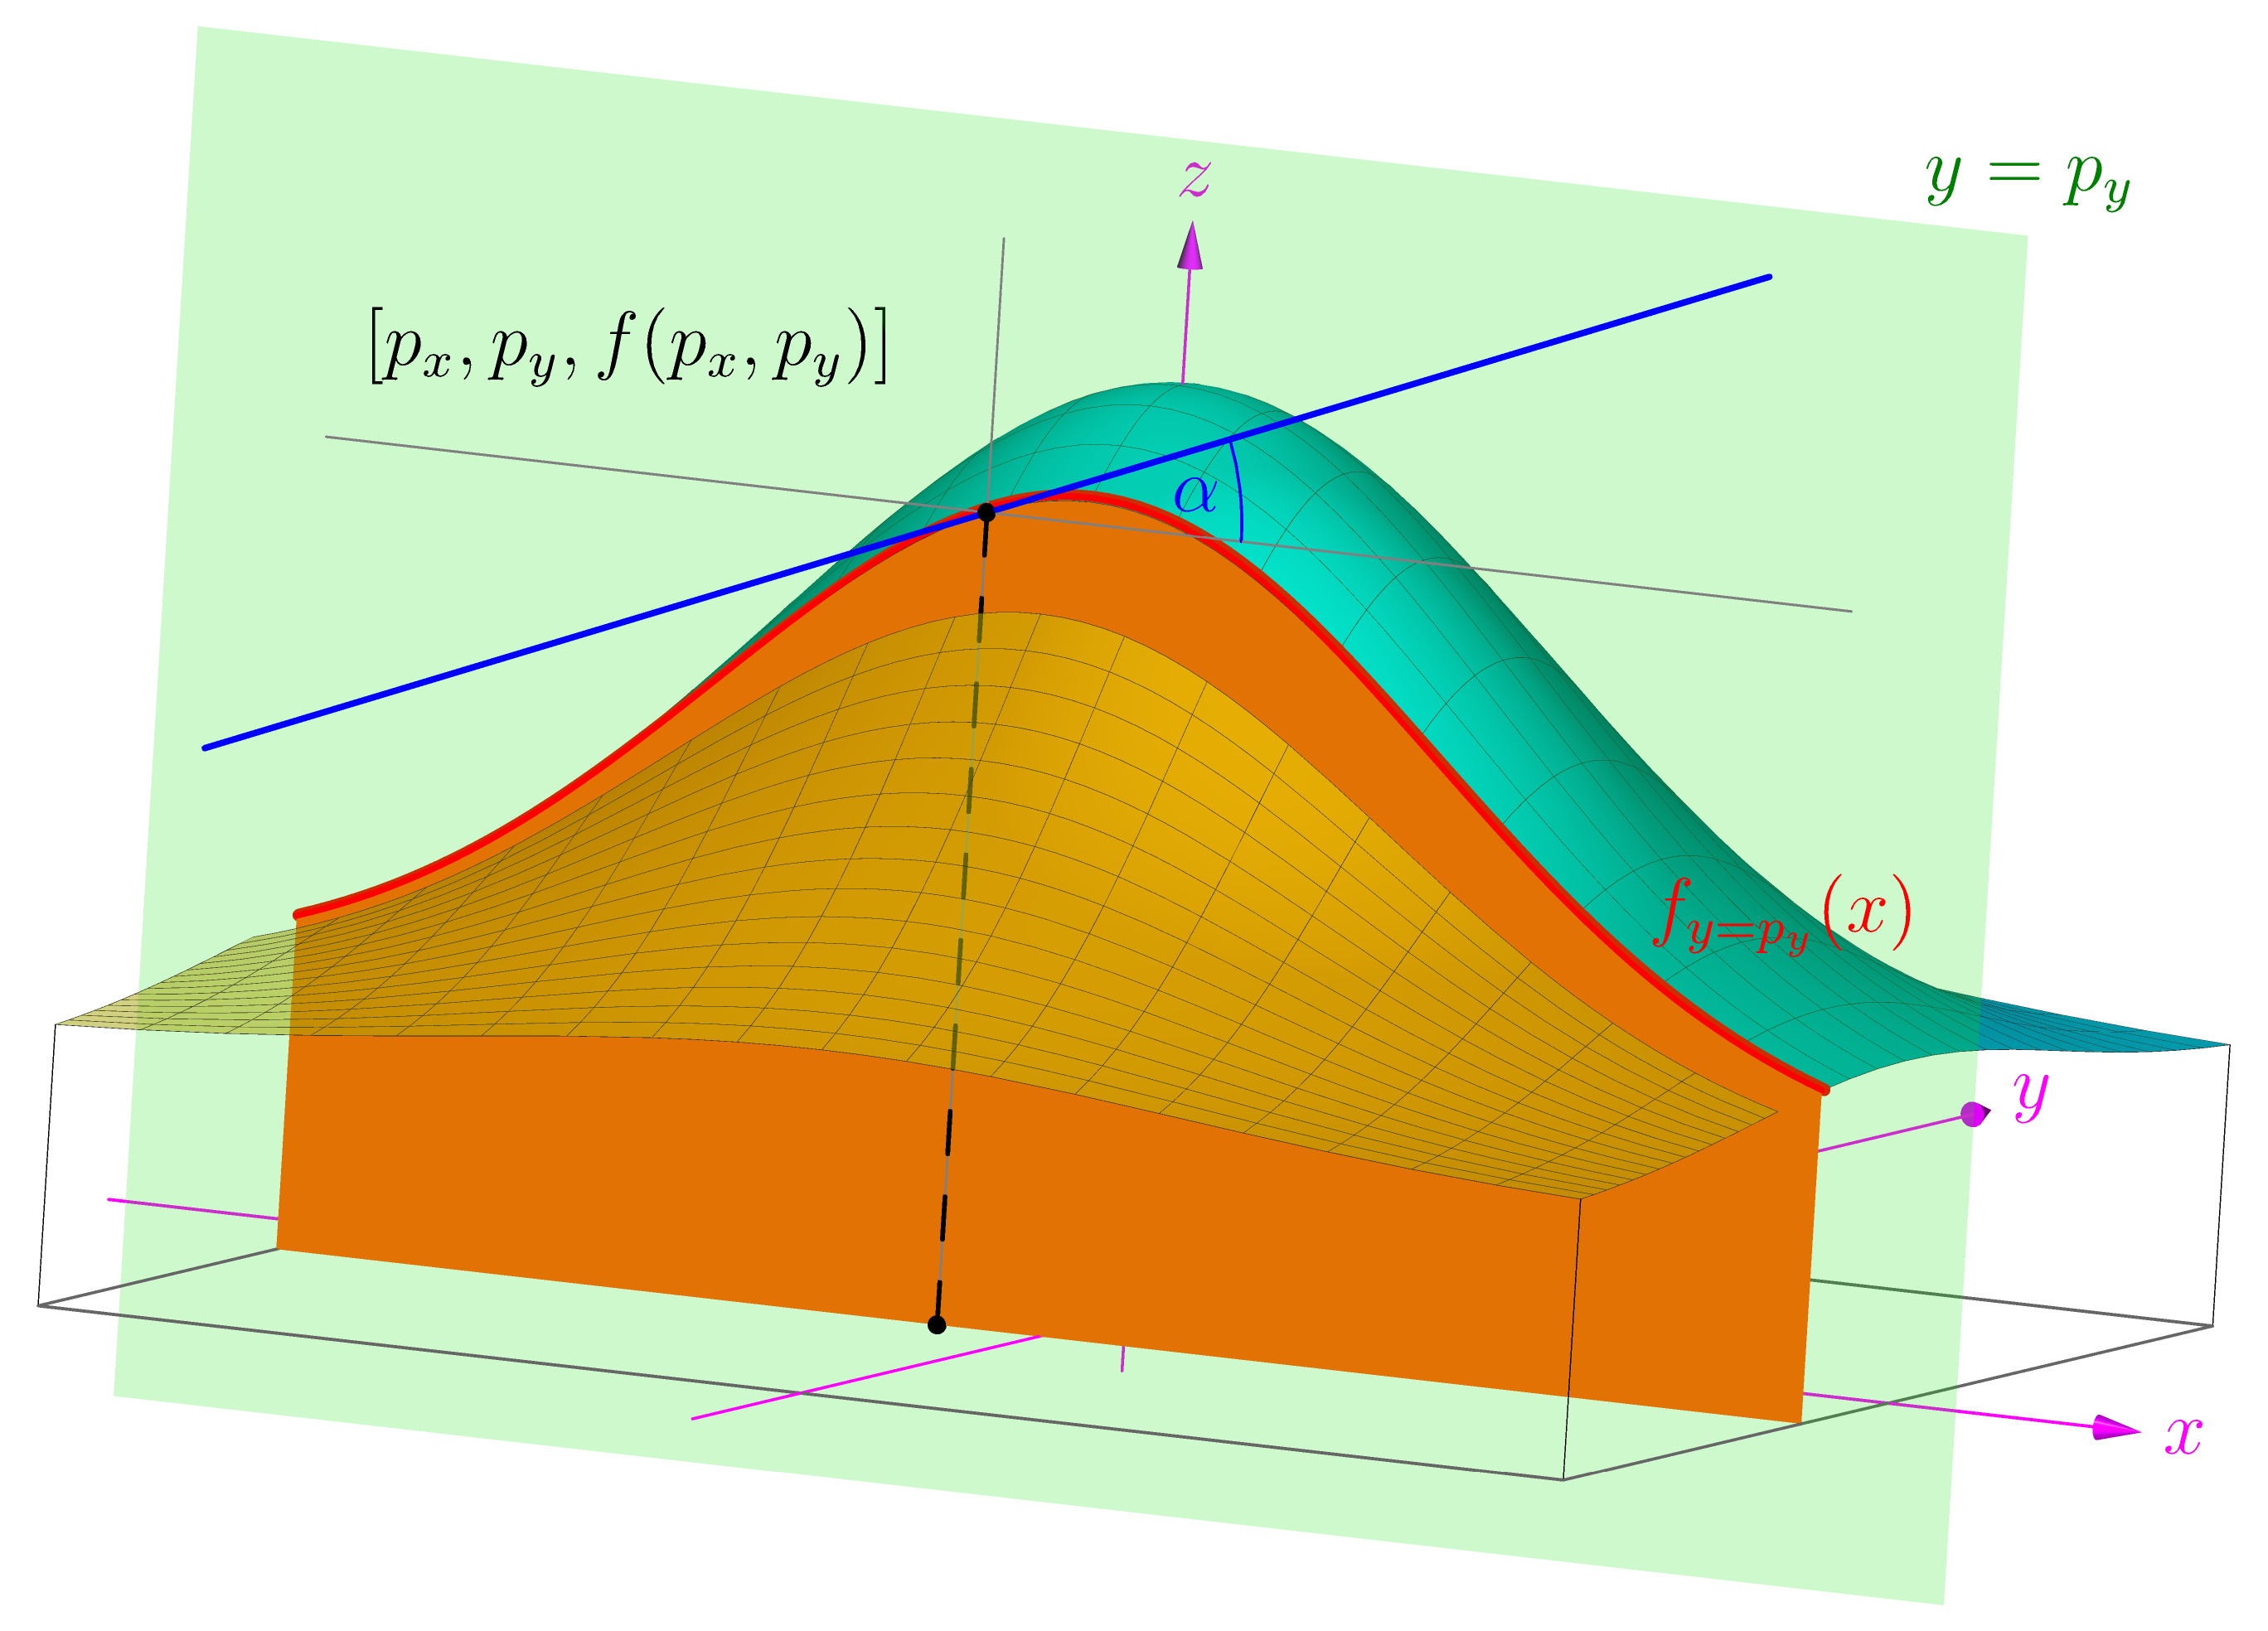
\includegraphics[width=12cm]{asy/partial1.png}}

Derivácia funkcie $f_{y=p_y}(x)$ v bode $p_x$ mi preto určuje, ako rastie výšková mapa
v bode $p$ v smere osi $x$. Toto je často používané číslo, preto  dostalo aj vlastný názov.\indexItem{Mat}{parciálna derivácia} 
Volá sa {\em parciálna derivácia} a zvykne sa označovať $\pdv{f}{x}(p)$.
To znamená, že keby som sa z bodu $p$ pohol o  veľmi malé $\Delta$ v smere 
osi $x$, tak hodnota $f(x,y)$ za zväčší o $\Delta\cdot\pdv{f}{x}(p)$.

Keď to podobne spravím pre os $y$, dostanem dva vektory $\vec{u}=\left[1,0,\pdv{f}{x}(p)\right]$ a  $\vec{v}=\left[0,1,\pdv{f}{y}(p)\right]$, ktoré mi určujú dotykovú rovinu
ku grafu funkcie $f$ v bode $\left[p_x,p_y,f(p_x,p_y)\right]$.

\centerline{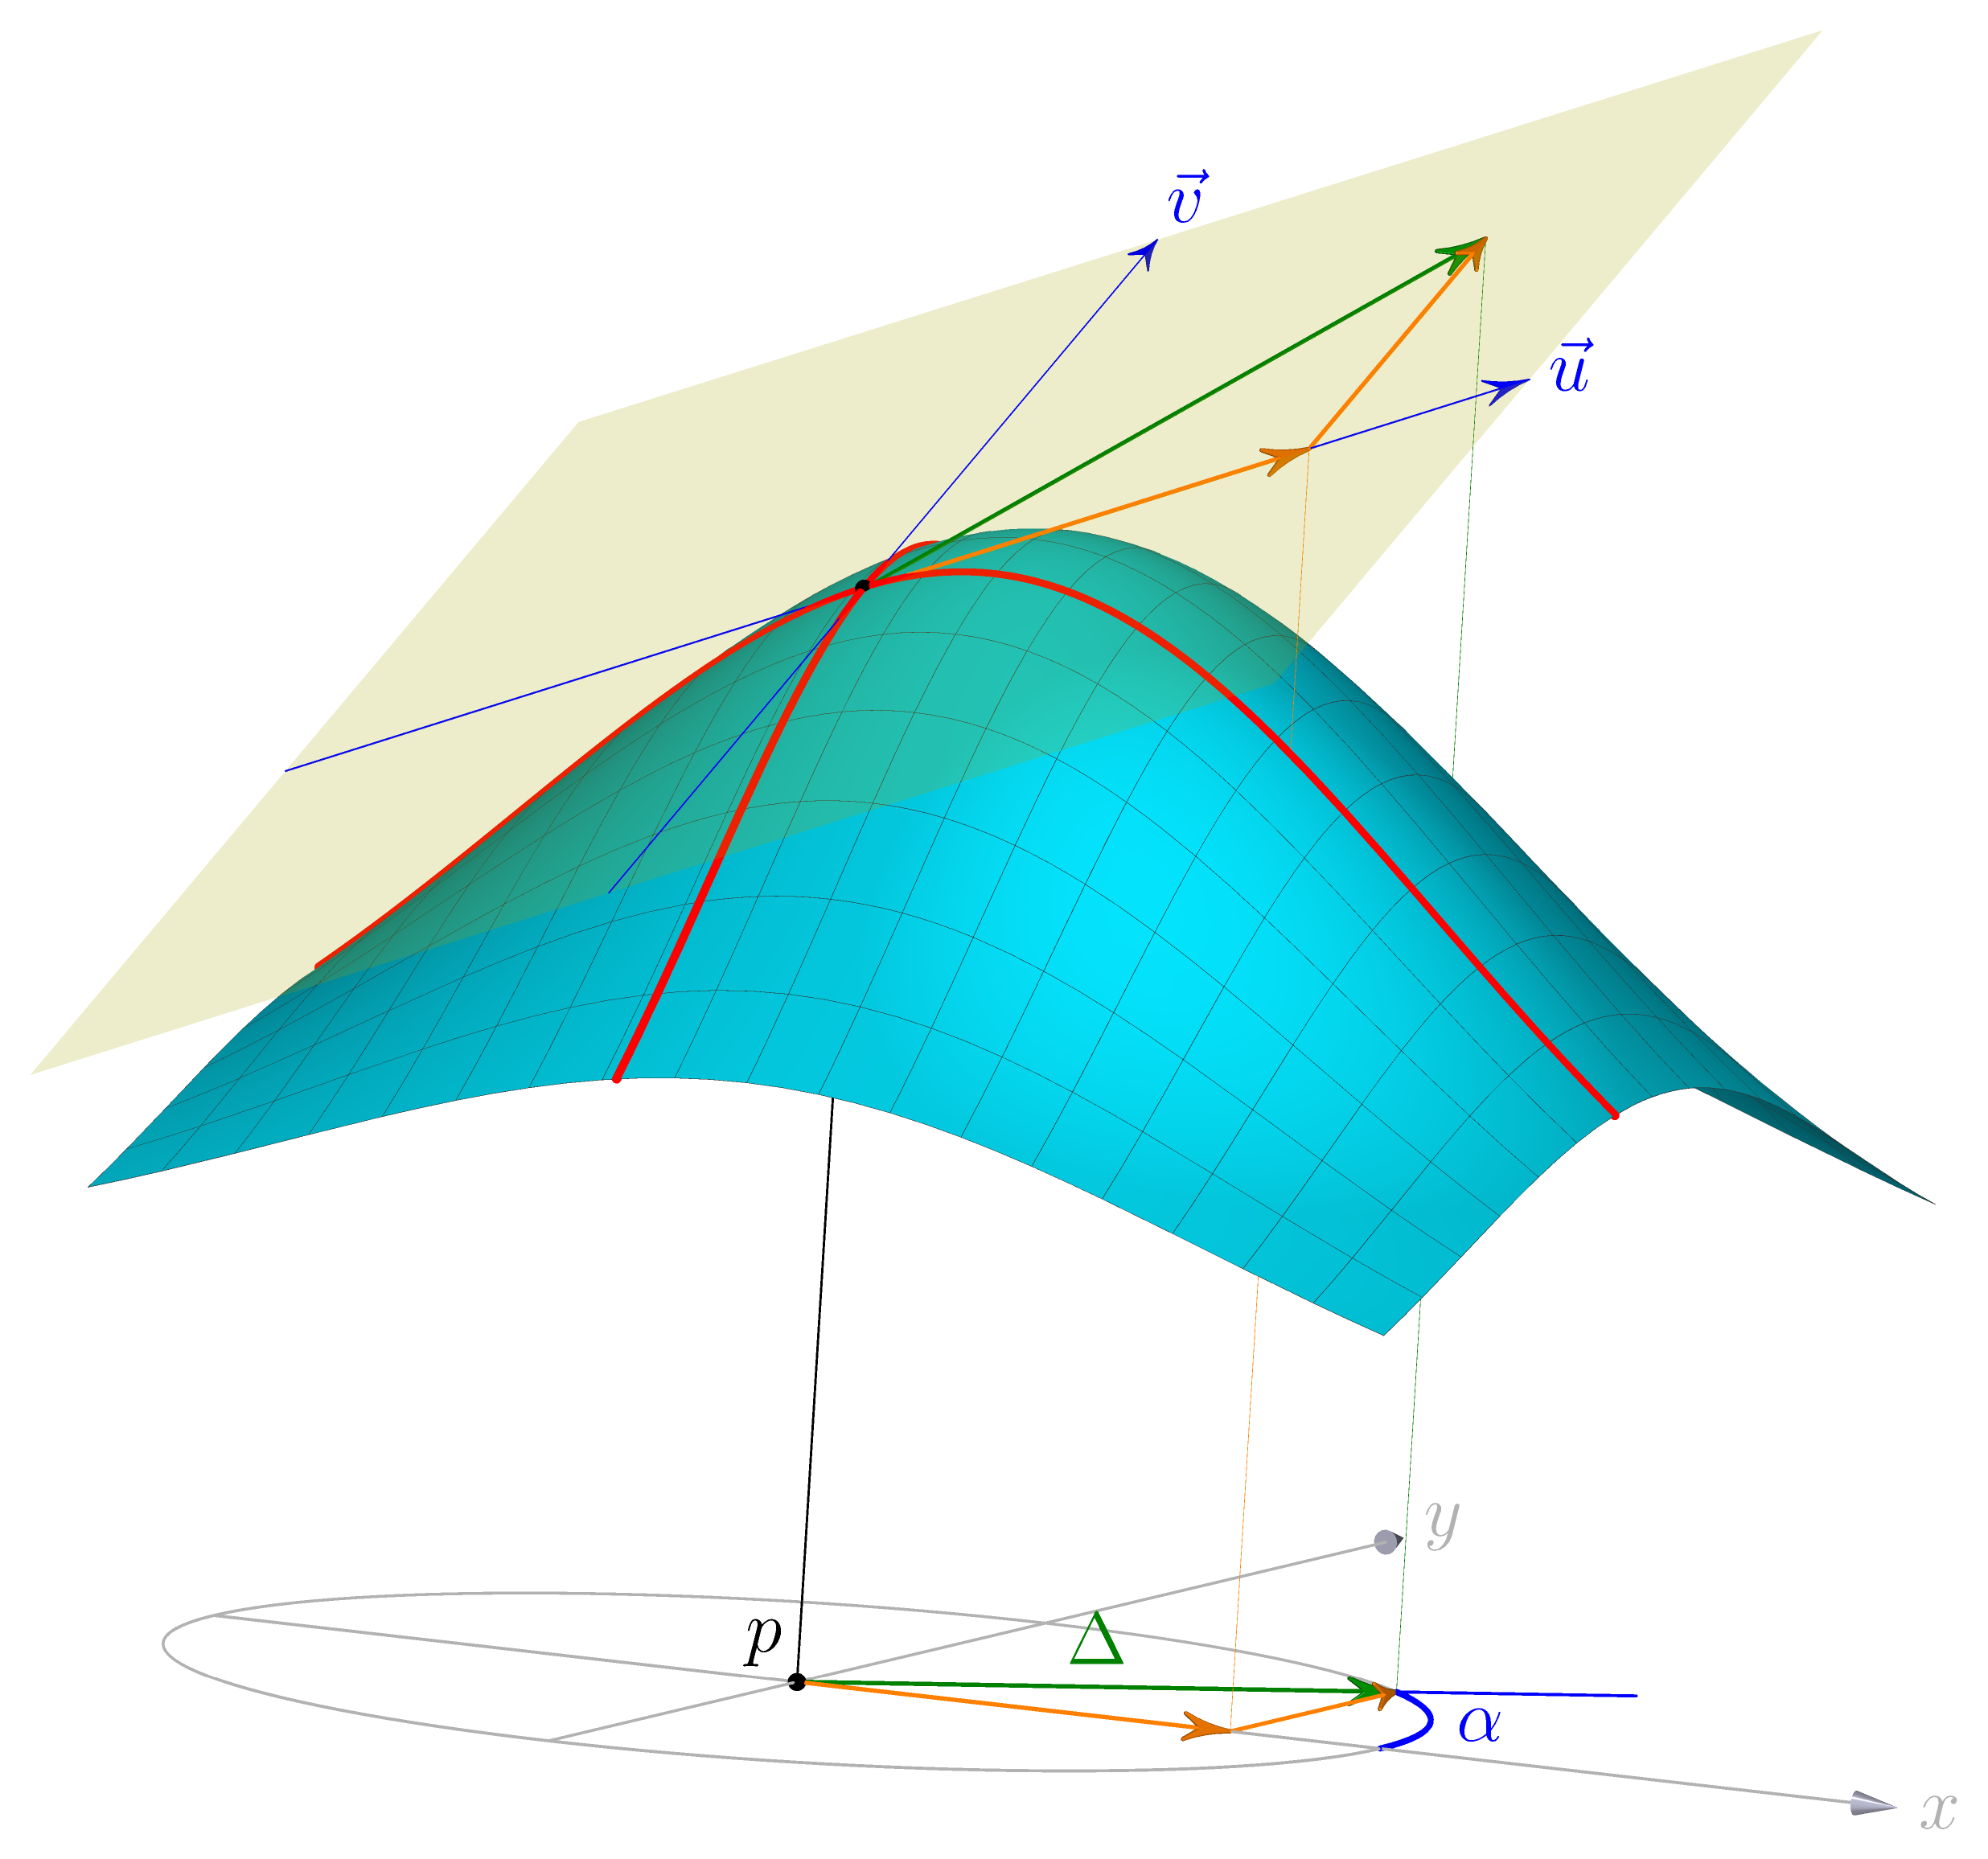
\includegraphics[width=11cm]{asy/partial2.png}}

Povedzme, že sa teraz pohnem z bodu $p$ o malý kúsok $\Delta$ pod uhlom $\alpha$. Zaujíma ma, ako sa zmení hodnota funkcie, ktorú si, ak je  $\Delta$ dosť malé, môžem nahradiť
dotykovou rovinou. Najprv sa pohnem v smere osi $x$ o $\Delta\cos(\alpha)$. Keďže v smere osi $x$ dotyková rovina rastie podľa vektora $\vec{u}$, 
hodnota narastie o $\Delta\cos(\alpha)\pdv{f}{x}(p_x,p_y)$. Potom sa pohnem v smere osi $y$ o $\Delta\sin(\alpha)$ a analogicky mi hodnota narastie o
$\Delta\sin(\alpha)\pdv{f}{x}(p_x,p_y)$. Keď to zrátam, dostanem, že keď som sa pohol o $\Delta$ pod uhlom $\alpha$, hodnota 
narástla o $\Delta\left(\cos(\alpha)\pdv{f}{x}(p_x,p_y)+\sin(\alpha)\pdv{f}{y}(p_x,p_y)\right)$.
Ak si označím $\vec{w}=\left[\cos(\alpha),\sin(\alpha)\right]$ vektor smeru o ktorý som sa pohol 
a $\vec\nabla=\left[\pdv{f}{x}(p_x,p_y),\pdv{f}{y}(p_x,p_y)\right]$ vektor parciálnych derivácií, vidím, že hodnota narástla o $\Delta(\vec{w}\cdot\vec{\nabla})$. A keď si pripomeniem,
čo sme rozprávali o skalárnom súčine na str.~\pageref{page:dotproduct-angle}, vidím, že hodnota narastie o
$\Delta\cdot\nrm{\vec{w}}\cdot\nrm{\vec{\nabla}}\cdot\cos(\varphi)$, kde $\varphi$ je uhol medzi vektormi $\vec{w}$ a $\vec{\nabla}$.

Akým smerom sa mám pohnúť, ak chcem, aby hodnota narástla čo najviac? Hodnoty $\Delta$, $\nrm{\vec{w}}$, $\nrm{\vec{\nabla}}$ sú stále rovnaké, jediné, čo sa mení, je
$\cos(\varphi)$. To znamená, že hodnota narastie najviac vtedy, keď $\cos(\varphi)$ bude $1$, t.j. keď $\varphi$ bude $0$. Inými slovami, hodnota narastie najviac
vtedy, keď sa pohnem v smere vektora $\vec{\nabla}$. 

Táto úvaha by sa dala zovšeobecniť aj na veľa rozmerov\footnote{To nie je úplne samozrejmé. Je veľa vecí, ktoré napr. platia v dvoch rozmeroch, ale v troch už nie (napr.
že dve priamky, ktoré nie sú rovnobežné, sa pretínajú), takže by bolo treba spraviť poriadny dôkaz pre veľa rozmerov. Tu ho ale neurobíme; išlo len o to ukázať intuíciu v pozadí.},
takže by sme dostali:


\begin{equation*}\boxed{\mathrm{Funkcia\ }n \mathrm{\ premenných\ } f(x_1,\ldots,x_n)
  \mathrm{\ rastie\ najrýchlejšie\ v\ smere\ vektora\ } gradientu \mathrm{\ }
\nabla=\left[\pdv{f}{x_1},\ldots,\pdv{f}{x_n}\right]}\end{equation*}

\vskip 1ex
Na záver matematickej odbočky si ešte raz všimni predchádzajúci obrázok. Máme tam funkciu $f(x,y)$
a jej dotykovú plochu v bode $p$. Čo by sa stalo, ak by $x$ a $y$ neboli premenné, ale 
nejaké funkcie parametra $t$, takže by nás zaujímala funkcia jednej premennej $h(t)=f(x(t),y(t))$?
Ako by vyzerala derivácia $\odv{h}{t}$? Ak parametrom $t$ pohnem o veľmi malé $\Delta$,
zmení sa hodnota $x(t)$ na  $x(t+\Delta)$. Keďže $\Delta$ je maličké, môžem si funkciu $x(t)$ nahradiť
jej dotyčnicou a dostanem $x(t+\Delta)\approx x(t)+\Delta\odv{x}{t}(t)$. Hodnota $y(t)$ sa podobne zmení na
$y(t+\Delta)\approx y(t)+\Delta\odv{y}{t}(t)$.
To znamená, že v dotykovej rovine k funkcii $f(x,y)$  
 sa pohnem o $\Delta\odv{x}{t}(t)$ v smere osi $x$ a hodnota funkcie
narastie o $\pdv{f}{x}(x(t),y(t))\Delta\odv{x}{t}(t)$. Potom sa pohnem 
o $\Delta\odv{y}{t}(t)$ v smere osi $y$ a hodnota funkcie narastie o ďalších $\pdv{f}{y}(x(t),y(t))\Delta\odv{y}{t}(t)$.
Dokopy teda ak pohnem parametrom $t$ o $\Delta$, hodnota $h(t)$ narastie o $\Delta\left(\pdv{f}{x}(x(t),y(t))\odv{x}{t}(t)+\pdv{f}{y}(x(t),y(t))\odv{y}{t}(t) \right)$.
Zasa by sa to dalo rozšíriť aj na viac rozmerov a dostali by sme analógiu derivácie zloženej funkcie pre viacero rozmerov:\indexItem{Mat}{derivácie zloženej funkcie vo viacerých rozmeroch}

\begin{equation*}\label{eq:diff_comp}\boxed{
    %\odv{f}{t}\left(g_1(t),g_2(t),\ldots,g_n(t)\right) = \sum_{i=1}^n\pdv{f}{g_i}\left(g_1(t),g_2(t),\ldots,g_n(t)\right)\cdot\odv{g_i}{t}(t)
    \begin{array}{c}
      \mathrm{Ak\ máme\ funkciu\ }f(x_1,\ldots,x_n) \mathrm{\ a\ } h(t)=f\left(g_1(t),g_2(t),\ldots,g_n(t)\right), \mathrm{\ potom\ }\\[1ex]
      \odv{h}{t}(t) = \sum\limits_{i=1}^n\pdv{f}{x_i}\left(g_1(t),\ldots,g_n(t)\right)\cdot\odv{g_i}{t}(t)
    \end{array}
}\end{equation*}


\def\err{\ensuremath{\mathrm{err}}}
\def\up#1{\ensuremath{^{(#1)}}}
\def\yh{\ensuremath{\widehat{\bm{Y}}}\xspace}
\vskip 2ex
Koniec matematickej odbočky, vráťme sa k našej jednoneurónovej ``sieti''. Povedali sme, že pre parametre $[w,b]$ je chyba siete $$\err(w,b)=\left(\tanh(wx_1+b)-y_1\right)^2.$$
Akým smerom treba pohnúť parametre, aby sa chyba čo najviac zmenšila? Teraz už vieme, že treba ísť v smere $-\nabla$, kde $\nabla$ je gradient
$\left[\pdv{\err}{w},\pdv{\err}{b}\right]$. Poďme teda rátať deriváciu. Funkciu $\tanh(\cdot)$ príliš nepoznáme, ale dá sa vyhľadať, že jej deriváciu už niekto zrátal a 
$$\tanh(x)'=\frac{1}{\cosh(x)^2}$$
$\cosh(\cdot)$ je nejaká iná funkcia, ktorá je dostupná z knižnice \vb{cmath} a to nám nateraz môže stačiť. Funkciu $\err$ si napíšeme ako zloženú funkciu takto

\begin{eqnarray*}
  \err(w,b) &=& \left(y(w,b)-y_1\right)^2\\
  y(w,b)&=&\tanh(u(w,b))\\
  u(w,b)&=&wx_1+b
\end{eqnarray*}

Použijeme, čo vieme o derivovaní zložených funkcií a napíšme si

\begin{align*}
  \pdv{\err}{w}=\pdv{\err}{y}\cdot\pdv{y}{u}\cdot\pdv{u}{w}& &
  \pdv{\err}{b}=\pdv{\err}{y}\cdot\pdv{y}{u}\cdot\pdv{u}{b}
\end{align*}

S tým, čo už vieme, zderivujeme jednotlivé funkcie ľahko:

\begin{align*}
  \pdv{\err}{y}=2(y-y_1)& &\pdv{y}{u}=\frac{1}{\cosh(u)^2}& &\pdv{u}{w}=x_1& &\pdv{u}{b}=1
\end{align*}

Keď to poskladáme dokopy, dostaneme

\begin{align*}
  \pdv{\err}{w}(w,b)=\frac{2x_1(\tanh(wx_1+b)-y_1)}{\cosh(wx_1+b)^2}& &
  \pdv{\err}{b}(w,b)=\frac{2(\tanh(wx_1+b)-y_1)}{\cosh(wx_1+b)^2}
\end{align*}

To znamená, že ak máme jednoneurónovú ``sieť'', tak pre akúkoľvek kombináciu 
$w$, $b$ vieme vyrátať, ktorým smerom treba hodnoty $w$ a $b$ pohnúť, aby sa chyba siete 
čo najrýchlejšie zmenšovala.


\vskip 1ex
Sieť s jedným neurónom nie je nič, čo by nás príliš uspokojilo, tak to poďme skúsiť zrátať 
pre zaujímavejšie siete. V našom programe máme triedu \vb{Network}, ktorá obsahuje pole vrstiev typu \vb{Layer}. 
Označme si vrstvy siete $L\up0,L\up1,\ldots,L\up{h-1}$. Každá vrstva obsahuje \vb{Matrix W,b}, tie vo vrstve $t$ si označme $\bm{W}\up{t}$, $\bm{b}\up{t}$.
Veľkosti vrstiev máme zapamätané vo \vb{vector<int> n}, takže $n_0$ je počet hodnôt na vstupe a $t$-ta vrstva $L\up{t}$ má $n_{t+1}$ neurónov,
takže $\bm{W}\up{t}$ je rozmerov $n_t\times n_{t+1}$ a $\bm{b}\up{t}$ je stĺpec $n_t\times1$. Tak, ako v predchádzajúcom hračkárskom príklade boli parametre siete
$w$ a $b$, teraz sú parametre všetky hodnoty vo všetkých
maticiach $\bm{W}\up{t}$, $\bm{b}\up{t}$. Podobne ako predtým, aj teraz potrebujeme zrátať chybu siete a potom gradient, t.j. deriváciu podľa každého z 
parametrov. Pripomeniem, že vyhodnocovanie vrstvy máme naprogramované takto:

\vskip 1ex
\vbox{
\begin{lstlisting}
Matrix Layer::eval(const Matrix &X) {
  Matrix res = W * X;
  res.addColumn(b);
  res.apply([](double x) { return tanh(x); });
  return res;
}
\end{lstlisting}}


Povedzme, že naša úloha má $s$ vstupov, takže vstupná matica $\bm{X}$ má rozmery $n_0\times s$. Prvá vrstva najprv 
vyráta $\bm{W}\up0\cdot\bm{X}$ a potom ku každému stĺpcu výsledku priráta $\bm{b}\up0$.
Tento medzivýsledok si označím $\bm{U}\up0$. Ak si označím $\bm{1}^s$ riadok obsahujúci $s$ jednotiek, ľahko sa overí, že $\bm{U}\up0=\bm{W}\up0\cdot\bm{X}+\bm{b}\up0\cdot\bm{1}^s$.
Nakoniec na každý prvok $\bm{U}\up0$ aplikujem $\tanh(\cdot)$. Túto operáciu budem označovať ako $\sigma\left(\bm{U}\up0\right)$ a výsledok označím $\bm{Y}\up0$.
Ak vstupom pre prvú vrstvu je vstupná matica $\bm{X}=\bm{X}\up0$, výstup z prvej vrstvy je vstupom pre druhú, t.j. $\bm{X}\up1=\bm{Y}\up0$.
Pri neurónových sieťach sa spravidla rozhodovacia funkcia neaplikuje na poslednú vrstvu, takže mám

\begin{align*}
  \bm{X}\up0&=\bm{X}\\
  \bm{U}\up{t}&=\bm{W}\up{t}\cdot\bm{X}\up{t}+\bm{b}\up{t}\cdot\bm{1}^s\\
  \bm{Y}\up{t}&=\sigma\left(\bm{U}\up{t}\right)\\
  \bm{X}\up{t+1}&=\bm{Y}\up{t}
\end{align*}


a dokopy sieť ráta zloženú funkciu

$$\bm{U}\up{h-1}=\bm{W}\up{h-1}\cdot\sigma\left(\bm{W}\up{h-2}\cdot\sigma\left(\cdots\sigma\left(\bm{W}\up0\cdot\bm{X}+\bm{b}\up0\cdot\bm{1}^s\right)\cdots\right)
+\bm{b}\up{h-2}\cdot\bm{1}^s\right)
+\bm{b}\up{h-1}\cdot\bm{1}^s$$


Ak si označím \yh maticu (rozmerov $h_{n-1}\times s$) správnych odpovedí, tak chyba siete, t.j. stredná kvadratická odchýlka, čiže priemer druhých mocnín rozdielov výstupných hodnôt a skutočných hodnôt, je


$$\err\left(\bm{W}\up0,\ldots,\bm{W}\up{h-1},\bm{b}\up0,\ldots,\bm{b}\up{h-1}\right)
=\frac{1}{s\cdot n_{h-1}}
\sum_{j=0}^{n_{h-1}}
\sum_{k=0}^{s-1}
\left(\yh_{j,k}-\bm{U}\up{h-1}_{j,k}\right)^2$$


$\err(\cdot)$ je veľmi zložitá funckia, v ktorej ako neznáme vystupujú všetky hodnoty z matíc $\bm{W}\up{t}$ a $\bm{b}\up{t}$. Aby sme zistili, ktorým smerom chyba najviac klesá, 
potrebujeme zrátať derivácie $\pdv{\err}{\bm{W}\up{t}_{j,k}}$ a $\pdv{\err}{\bm{b}\up{t}_j}$ pre všetky prípustné kombinácie $j$, $k$, $t$. 
Začneme s tým, že si pre všetky prípustné hodnoty $j$, $k$, $t$ vyrátame $\pdv{\err}{\bm{U}\up{t}_{j,k}}$.
\indexItem{Alg}{back propagation}
Pôjdeme pritom odzadu\footnote{preto sa táto metóda zvykne volať {\em back propagation}}. Pre fixné $j$, $k$ zrátame hodnotu $\pdv{\err}{\bm{U}\up{h-1}_{j,k}}$ tak,
že si predstavíme $\err$ ako funkciu jedinej premennej $\bm{U}\up{h-1}_{j,k}$ a zrátame deriváciu. Keď si rozpíšem zápis so sumami, dostanem

$$\err = \frac{1}{s\cdot n_{h-1}}\left(\yh_{0,0}-\bm{U}\up{h-1}_{0,0}\right)^2+\cdots+
 \frac{1}{s\cdot n_{h-1}}\left(\yh_{j,k}-\bm{U}\up{h-1}_{j,k}\right)^2+\cdots+
 \frac{1}{s\cdot n_{h-1}}\left(\yh_{n_{h-1},s-1}-\bm{U}\up{h-1}_{n_{h-1},s-1}\right)^2
$$

Už vieme, že derivácia konštantnej funkcie je $0$ a $\left(f(x)+g(x)\right)'=f'(x)+g'(x)$. V predchádzajúcom výraze je jediný člen, ktorý závisí od $\bm{U}\up{h-1}_{j,k}$, preto
všetko ostatné sa zderivuje na nulu a ostane mi

$$\pdv{\err}{\bm{U}\up{h-1}_{j,k}}=\frac{-2}{s\cdot n_{h-1}}\left(\yh_{j,k}-\bm{U}\up{h-1}_{j,k}\right)$$

Predstavme si teraz, že už máme pre nejaké $t$ zrátané $\pdv{\err}{\bm{U}\up{t+1}_{j,k}}$ pre všetky 
$j$, $k$ a chceme z nich vyrátať $\pdv{\err}{\bm{U}\up{t}_{j,k}}$.
Pretože $\bm{Y}\up{t}_{j,k}=\sigma\left(\bm{U}\up{t}_{j,k}\right)$ vždy aplikuje $\tanh(\cdot)$ na 
jednotlivé prvky v matici $\bm{U}$, predstavím si to ako zloženú funkciu a môžem si vyjadriť

$$\pdv{\err}{\bm{U}\up{t}_{j,k}}=
\pdv{\err}{\bm{Y}\up{t}_{j,k}}\cdot\odv{\bm{Y}\up{t}_{j,k}}{\bm{U}\up{t}_{j,k}}$$

pričom $\odv{\bm{Y}\up{t}_{j,k}}{\bm{U}\up{t}_{j,k}}$ je derivácia $\tanh(\cdot)$,
teda
$$ \odv{\bm{Y}\up{t}_{j,k}}{\bm{U}\up{t}_{j,k}}=\frac{1}{\cosh\left(\bm{U}\up{t}_{j,k}\right)^2}$$ 


Teraz chceme zrátať pre premennú $\bm{Y}\up{t}_{j,k}$ hodnotu $\pdv{\err}{\bm{Y}\up{t}_{j,k}}$, ak už máme zrátané všetky hodnoty $\pdv{\err}{\bm{U}\up{t+1}_{\ell,r}}$.
Na to použijeme rámček o zložených funkciách zo strany~\pageref{eq:diff_comp}: Najprv si predstavím, 
že $\err$ je funkcia premenných $\bm{U}\up{t+1}_{\ell,r}$
a potom si poviem, že v skutočnosti $\bm{U}\up{t+1}_{\ell,r}$ závisia od premenných $\bm{Y}\up{t}_{j,k}$, preto

$$\pdv{\err}{\bm{Y}\up{t}_{j,k}}=\sum_{\ell<n_{t+1}}\sum_{r<s}\pdv{\err}{\bm{U}\up{t+1}_{\ell,r}}\cdot\pdv{\bm{U}\up{t+1}_{\ell,r}}{\bm{Y}\up{t}_{j,k}}$$

Treba nám preto zistiť, ako závisí $\bm{U}\up{t+1}_{\ell,r}$ od $\bm{Y}\up{t}_{j,k}$.
Vieme, že $\bm{U}\up{t+1}=\bm{W}\up{t+1}\cdot\bm{Y}\up{t}+\bm{b}\up{t+1}\cdot\bm{1}^s$.
Keď si nakreslíme príslušné matice aj s ich rozmermi, bude to vyzerať takto:

\vskip 1ex
\centerline{
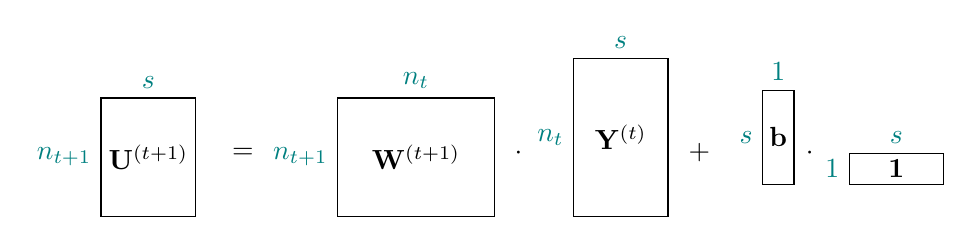
\begin{tikzpicture}
  \def\mtx#1[#2]#3[#4]#5{
    \draw(0,0) rectangle node{$#5$}(#2,#4);
    \draw[teal,draw=none](0,0) -- node[anchor=east]{$#3$}(0,#4);
    \draw[teal,draw=none](0,#4) -- node[anchor=south]{$#1$}(#2,#4);
  }

  \begin{scope}[shift={(-3,0)}]
    \mtx{s}[1.2]{n_{t+1}}[1.5]{\bm{U}\up{t+1}}
  \end{scope}
  
  \node at (-1.2,0.8) {$=$};


  \mtx{n_t}[2]{n_{t+1}}[1.5]{\bm{W}\up{t+1}}
  
  \node at (2.3,0.8) {$\cdot$};
  
  \begin{scope}[shift={(3,0)}]
    \mtx{s}[1.2]{n_t}[2]{\bm{Y}\up{t}}
  \end{scope}
  
  \node at (4.6,0.8) {$+$};
  
  \begin{scope}[shift={(5.4,0.4)}]
    \mtx{1}[0.4]{s}[1.2]{\bm{b}}
  \end{scope}
  \node at (6,0.8) {$\cdot$};
  \begin{scope}[shift={(6.5,0.4)}]
    \mtx{s}[1.2]{1}[0.4]{\bm{1}}
  \end{scope}

\end{tikzpicture}}

To znamená, že $$\bm{U}\up{t+1}_{\ell,r}=\sum_{i=0}^{n_t-1}\bm{W}\up{t+1}_{\ell,i}\bm{Y}\up{t}_{i,r}+\bm{b}\up{t+1}_\ell$$

Keďže nás zaujíma iba to, ako $\bm{U}\up{t+1}_{\ell,r}$ závisí od $\bm{Y}\up{t}_{j,k}$, vidíme, že ak $r\not=k$, tak $\bm{Y}\up{t}_{j,k}$ 
v tomto výraze nevystupuje a pre $r=k$ si môžeme  napísať

\def\oblacik{\raisebox{-0.6ex}{\usymH{1F5F0}{2.8ex}}\xspace}

$$\bm{U}\up{t+1}_{\ell,k}=\bm{W}\up{t+1}_{\ell,j}\bm{Y}\up{t}_{j,k}+\oblacik$$

pričom \oblacik od $\bm{Y}\up{t}_{j,k}$ nezávisí. Preto 
$\pdv{\bm{U}\up{t+1}_{\ell,k}}{\bm{Y}\up{t}_{j,k}}=\bm{W}\up{t+1}_{\ell,j}.$
Keď sa vrátime o krok späť, dostaneme

$$\pdv{\err}{\bm{Y}\up{t}_{j,k}}=\sum_{\ell<n_{t+1}}\pdv{\err}{\bm{U}\up{t+1}_{\ell,k}}\cdot\bm{W}\up{t+1}_{\ell,j}$$

\def\uh{\ensuremath{\widehat{\bm{U}}}\xspace}
\def\wh{\ensuremath{\widehat{\bm{W}}}\xspace}

Keď sa pozornejšie prizrieš, čo sme zrátali, pripomína to násobenie matíc. Ak si označím $\uh\up{t+1}$ maticu rozmerov $n_{t+1}\times s$, ktorá
bude obsahovať hodnoty $\pdv{\err}{\bm{U}\up{t+1}_{\ell,r}}$
a $\yh\up{t}$ maticu rozmerov $n_t\times s$, 
ktorá
bude obsahovať hodnoty $\pdv{\err}{\bm{Y}\up{t}_{j,k}}$, tak

$$\yh\up{t}=\bm{W}\tran{}\up{t+1}\cdot\uh\up{t+1}$$

Uff. Tak toto bolo trochu viac rátania, ale o to jednoduchšie budeme mať teraz programovanie. Triedu \vb{Layer} si prerobím tak, že si bude okrem matíc \vb{W} a \vb{b}
pamätať aj \vb{U}, \vb{Y} a \vb{dU}, čo budú naše matice $\bm{U}\up{t}$, $\bm{Y}\up{t}$ a $\uh\up{t}$.

\vskip 1ex
\vbox{
\begin{lstlisting}
struct Layer {
  int n1;       // počet neurónov vo vrstve
  int n0;       // veľkosť predchádzajúcej vrstvy (vstupu)
  Matrix W, b;  // W: n1 x n0, kde w[i,j] = váha i-teho neurónu k j-temu vstupu
                // b: stĺpec n1 x 1
  Matrix U, Y;  // n1 x s : výstupné hodnoty neurónov pred a po aktivácii
  Matrix dU;    // derivácia chyby podľa U
                
  Layer(int _n0, int _n1);   // konštruktor

  void feed(const Matrix&);                // spracuj vstup, nastav U
  void activate();                         // nastav Y podľa už nastaveného U
  void backPropagation(const Layer& nxt);  // nastav dU podľa nasledujúcej vrstvy
};
\end{lstlisting}
}



Jednotlivé metódy sa napíšu priamočiaro:

\vskip 1ex
\vbox{
\begin{lstlisting}
void Layer::feed(const Matrix &x) {
  if (x.m != s) {
    s = x.m;
    U = Matrix(n1, s);
  }
  multInto(W, x, U);
  U.addColumn(b);
}
\end{lstlisting}
}


\vskip 1ex
\vbox{
\begin{lstlisting}
void Layer::activate() {
  Y = U;
  Y.apply([](double x) { return tanh(x); });
}
\end{lstlisting}
}

\vskip 1ex
\vbox{
\begin{lstlisting}
void Layer::backPropagation(const Layer &nxt) {
  Matrix Z = (nxt.W.transposed()) * nxt.dU;
  dU = U;
  dU.apply([this](Num x) { 
      Num tmp = cosh(x);
      return 1.0 / (tmp * tmp);
  });
  dU.fill([this, &Z](int i, int j) { return dU(i, j) * Z(i, j); });
}
\end{lstlisting}
}


Metóda \vb{backPropagation} vyráta \vb{dU} v jednej vrstve na základe už vyrátanej \vb{dU} z nasledujúcej vrstvy.
Aby to celé mohlo odštartovať, potrebujeme zrátať \vb{dU} v poslednej vrstve. V nej rátame chybu pomocou \vb{mse},
takže si spravíme takúto funkciu, ktorá vyráta $\pdv{\err}{\bm{U}\up{h-1}_{j,k}}$ a výsledok uloží v matici \vb{D}:

\vskip 1ex
\vbox{
\begin{lstlisting}
void diffMse(const Matrix &data, const Matrix &truth, Matrix &D) {
    const int n = truth.n, m = truth.m;
    if (D.n != n || D.m != m) D = Matrix(n, m); // prerob ak nemá správne rozmery
    for (int i = 0; i < n; i++)
        for (int j = 0; j < m; j++)
            D(i, j) = -2.0 / (double)(n * m) * (truth(i, j) - data(i, j));
}
\end{lstlisting}
}

Celá sieť bude vstup spracovávať v metóde \vb{feed}, ktorá výsledok uloží v \hbox{\vb{layers[h - 1].U}}:

\vskip 1ex
\vbox{
\begin{lstlisting}
Matrix& Network::feed(const Matrix &input) {
  const Matrix *x = &input;
  for (int i = 0; i < h - 1; i++) {
    layers[i].feed(*x);
    layers[i].activate();
    x = &layers[i].Y;
  }
  layers[h - 1].feed(*x);
  return layers[h - 1].U;
}

Matrix& Matrix::output() { return layers[h - 1].U; }

Num Network::error(const Matrix &output, const Matrix &truth) { 
  return mse(output, truth); 
}
\end{lstlisting}
}

Volanie \vb{Network::backPropagation} najprv nechá vstupnú maticu prejsť vrstvu po vrstve 
cez celú sieť metódou \vb{feed}, ktorá v každej vrstve nastaví hodnoty \vb{U} a \vb{Y}. 
Potom v opačnom poradí nastaví v každej vrstve \vb{dU}. 

\vskip 1ex
\vbox{
\begin{lstlisting}
void Network::backPropagation(const Matrix &input, const Matrix &truth) {
  feed(input);
  diffMse(layers[h - 1].U, truth, layers[h - 1].dU);
  for (int i = h - 2; i >= 0; i--) layers[i].backPropagation(layers[i + 1]);
}
\end{lstlisting}
}


Stále ešte ale nemáme zrátaný gradient,
t.j. hodnoty $\pdv{\err}{\bm{W}\up{t}_{j,k}}$ a $\pdv{\err}{\bm{b}\up{t}_j}$.
Keď už ale máme zrátané $\pdv{\err}{\bm{U}\up{t}_{j,k}}$, tento zvyšok dorátame ľahko.
Vieme, že
$$\bm{U}\up{t}=\bm{W}\up{t}\cdot\bm{Y}\up{t-1}+\bm{b}\up{t}\cdot\bm{1}\up{s}$$
Pozrime sa najprv na tú ťažšiu vec, na $\pdv{\err}{\bm{W}\up{t}_{j,k}}$. Podobne, ako pred chvíľou,
predstavím si $\err$ ako zloženú funkciu premenných $\bm{U}\up{t}_{\ell,r}$, ktoré v skutočnosti závisia
od $\bm{W}\up{t}_{j,k}$ a dostanem
$$\pdv{\err}{\bm{W}\up{t}_{j,k}}=\sum_{\ell<n_t}\sum_{r<s}
\pdv{\err}{\bm{U}\up{t}_{\ell,r}}\cdot\pdv{\bm{U}\up{t}_{\ell,r}}{\bm{W}\up{t}_{j,k}}.$$

Pretože 
$$\bm{U}\up{t}_{\ell,r}=\sum_{i=0}^{n_t-1}\bm{W}\up{t}_{\ell,i}\bm{Y}\up{t-1}_{i,r}+\bm{b}\up{t}_\ell$$
tak viem, že $\bm{U}\up{t}_{\ell,r}$ závisí od môjho $\bm{W}\up{t}_{j,k}$
iba vtedy, keď $l=j$, a potom

$$\bm{U}\up{t}_{j,r}=\bm{W}\up{t}_{j,k}\bm{Y}\up{t-1}_{k,r}+\oblacik$$


$$\pdv{\err}{\bm{W}\up{t}_{j,k}}=
\sum_{r<s}\pdv{\err}{\bm{U}\up{t}_{j,r}}\cdot
\pdv{\bm{U}\up{t}_{j,r}}{\bm{W}\up{t}_{j,k}}=
\sum_{r<s}\pdv{\err}{\bm{U}\up{t}_{j,r}}\cdot
\bm{Y}\up{t-1}_{j,k}
$$


Opäť, ak si označím $\wh\up{t}$ maticu, kde budú hodnoty $\pdv{\err}{\bm{W}\up{t}_{j,k}}$,
tak 
$$ \wh\up{t}=\uh\up{t}\cdot\bm{Y}\bm\tran{}\up{t-1}$$

S hodnotami $\pdv{\err}{\bm{b}\up{t}_j}$ je to ešte jednoduchšie, lebo mám výraz

$$\pdv{\err}{\bm{b}\up{t}_{j}}=\sum_{\ell<n_t}\sum_{r<s}
\pdv{\err}{\bm{U}\up{t}_{\ell,r}}\cdot\pdv{\bm{U}\up{t}_{\ell,r}}{\bm{b}\up{t}_{j}}$$
a $\bm{U}\up{t}_{\ell,r}=\bm{b}\up{t}_\ell+\oblacik$.

Takže to môžeme rovno doprogramovať. Urobíme to tak, že potom, čo sa zavolá 
\hbox{\vb{Network::backPropagation()}} a nastavia sa \vb{dU} vo všetkých vrstvách, zavoláme 
\vb{Network::gradient()}, ktorý vyráta matice \vb{dW} a \vb{db} pre každú vrstvu.
Môžem si to spraviť tak, že každá vrstva vráti matice \vb{dW} a \vb{db}
v jednom type \vb{LayerData}. Pridané funkcie budú vyzerať nejak takto:

\vskip 1ex
\vbox{
\begin{lstlisting}
struct LayerData {
  Matrix dW, db;
};

using Gradient = std::vector<LayerData>;
\end{lstlisting}
}

\vskip 1ex
\vbox{
\begin{lstlisting}
LayerData Layer::gradient(const Matrix &Y) {
  LayerData res{dU * Y.transposed(), Matrix(n1, 1)};
  for (int j = 0; j < n1; j++) {
    res.db(j, 0) = 0;
    for (int k = 0; k < s; k++) res.db(j, 0) += dU(j, k);
  }
  return res;
}
\end{lstlisting}
}

\vskip 1ex
\vbox{
\begin{lstlisting}
Gradient Network::gradient(const Matrix &input) {
  Gradient res(h);
  for (int i = h - 1; i > 0; i--)
    res[i] = std::move(layers[i].gradient(layers[i - 1].Y));
  res[0] = std::move(layers[0].gradient(input));
  return res;
}
\end{lstlisting}
}

\vskip 1ex
\vbox{
\begin{lstlisting}
void Network::apply(Num a, const Network::Gradient &g) {
  for (int t = 0; t < h; t++) {
    layers[t].W.addMultiple(-a, g[t].dW);
    layers[t].b.addMultiple(-a, g[t].db);
  }
}
\end{lstlisting}
}

Pri trénovaní siete to potom vyzerá takto:

\vskip 1ex
\vbox{
\begin{lstlisting}
net.backPropagation(data, truth);
auto err = net.error(net.output(), truth);
auto g = net.gradient(data);
net.apply(step, g);
\end{lstlisting}
}

V riadku $2$ som si zrátal chybu, ktorú môžem použiť napríklad na to, aby som vedel, kedy s trénovaním prestať.
Parameter \vb{step} mi hovorí, koľko z gradientu mám prirátať, t.j. ako ďaleko sa v smere gradientu pohnem.
Zvoliť ho je celkom umenie: ak je príliš veľký, pôjdem v smere gradientu priďaleko a chyba siete narastie. Ak je 
príliš malý, trénovanie bude trvať pridlho. Môžeš si skúsiť rozmyslieť spôsob, ako \vb{step} automaticky meniť
(napr. ak chyba klesla, tak ho trochu zväčšiť, ak stúpla, tak ho zmenšiť).

\begin{uloha}
  Naprogramuj sieť, ktorá sa učí pomocou {\em back propagation} a otestuj ju
  na našom príklade s prvočíslami.
\end{uloha}


Keď som spúšťal túto vylepšenú sieť na príklade s 8-bitovými prvočíslami, kde 
náhodné učenie trvalo okolo 80000 iterácií, tak back propagation bolo spravidla veľmi rýchle, ale občas,
ak náhodné nastavenie siete na začiatku dopadlo nejak zle, učenie trvalo dlho. Preto som si povedal,
že ak sieť počíta viac ako 5000 iterácií a chyba je stále priveľká, sieť zahodím a skúsim to celé od začiatku. Vo výsledku mi stačilo v priemere 
4300 iterácií. To je oveľa menej, ako 80000 iterácií pri náhodnom učení, a pre väčšie siete by ten rozdiel bol ešte väčší.
Zároveň je vidieť, že čas stále dosť závisel od toho, ako sa na začiatku 
sieť náhodne nastavila.

\vskip 2ex
\newtoks\mycoords
\mycoords{}

\foreach \x[count=\i from 1] in {4347,	2605,	6875,	3398,	2148,	2484,	11775,	2271,	8771,	1589,
3800,	7184,	2090,	1525,	4532,	6852,	9574,	2967,	2352,	8491,	1492,	2299,	1386,
2270,	2159,	2283,	1457,	2510,	3262,	1935,	2743,	2942,	6819,	2515,	7495,	3858,
6532,	2170,	4869,	6920,	7581,	2394,	8506,	14079,	1805,	3558,	2756,	1523,	2468,
6641} {\global\mycoords\expandafter{%
  \expanded{\the\mycoords(\i,\x)}} }

\centerline{
\begin{tikzpicture}
  \begin{axis}[
      width=\textwidth, height=6cm, xmin=0, xmax=51, 
      ybar=0pt, bar width=2mm,  xtick=data, xticklabel=\empty,
       /pgf/number format/fixed,
       scaled y ticks=false,
      %1000 sep={}
   ]
    \addplot[ybar,fill=teal!50!white] coordinates {\the\mycoords};
  \end{axis}
\end{tikzpicture}}

\vskip 1ex
Doteraz sme sieť používali tak, že sme na nájdenie váh neurónov (a.k.a. {\em trénovanie}) použili všetky možné vstupy a výstupy úlohy. Čo ale s úlohami, ktoré majú 
priveľa možných vstupov? Urobíme to tak, že si vyberieme niekoľko vstupov a natrénujeme sieť iba na nich. Týmto nedostaneme presné riešenie úlohy, lebo o vstupoch, ktoré sme na
trénovanie nepoužili, nevieme nič. Môžeme sa ale spoliehať na to, že veľa úloh má takú vlastnosť, že vstupy, ktoré sú v istom zmysle podobné,
budú mať aj podobné riešenie. A rovnakú vlastnosť má aj neurónová sieť: na podobné vstupy dáva podobnú odpoveď. Ako dobre to môže fungovať závisí od konkrétnej úlohy. 
Poďme si to vyskúšať na jednoduchom príklade. Dajme tomu, že chcem mať sieť s dvoma vstupnými neurónmi, ktoré budú mať hodnoty medzi $-1$ a $1$. Tieto vstupné hodnoty sú súradnice
bodu v rovine a mojím cieľom je povedať, akú farbu má bod s danými súradnicami v tomto vzore:

\def\dim{2.5cm}
\vskip 1ex

{%
\setlength{\fboxsep}{0pt}%
\setlength{\fboxrule}{0.2pt}%
\centerline{\fbox{
\includegraphics[width=\dim]{data/netsamples/square2.png}}}
}

Zobral  som si  dve siete. Jedna mala tri vrstvy s 2, 5 a jedným neurónom a druhá tri vrstvy s 2, 80,
80 a jedným neurónom. Potom som pre rôzne počty nádodne vybratých bodov natrénoval obe siete a
následne sa pozrel, aké odpovede dávali pre ostatné body.

\def\ms#1{%
{%
\setlength{\fboxsep}{0pt}%
\setlength{\fboxrule}{0.2pt}%
\raisebox{-1.25cm}{\fbox{\includegraphics[width=\dim]{data/netsamples/square2_2_5_1_sz0#1_dots.png}}}
}
}
\def\vs#1{%
{%
\setlength{\fboxsep}{0pt}%
\setlength{\fboxrule}{0.2pt}%
\raisebox{-1.25cm}{\fbox{\includegraphics[width=\dim]{data/netsamples/square2_2_80_80_1_sz0#1_dots.png}}}
}
}

\begin{column}{0.45}
\begin{tblr}{
  colspec = {Q[m,c]Q[m,c]Q[m,c]},
  stretch = 0,
  rowsep = 6pt,
  hline{1,Z} = {1pt},
  hline{2} = {0.5pt},
}
  vzorky& \vb{2,5,1} & \vb{2,80,80,1} \\
  10 & \ms{0010} & \vs{0010} \\
  40 & \ms{0040} & \vs{0040} \\
  60 & \ms{0060} & \vs{0060} \\
  100 & \ms{0100} & \vs{0100} \\
  150 & \ms{0150} & \vs{0150} \\
\end{tblr}
\end{column}
\hfill
\begin{column}{0.45}
\begin{tblr}{
  colspec = {Q[m,c]Q[m,c]Q[m,c]},
  stretch = 0,
  rowsep = 6pt,
  hline{1,Z} = {1pt},
  hline{2} = {0.5pt},
}
  vzorky& \vb{2,5,1} & \vb{2,80,80,1} \\
  200 & \ms{0200} & \vs{0200} \\
  300 & \ms{0300} & \vs{0300} \\
  400 & \ms{0400} & \vs{0400} \\
  600 & \ms{0600} & \vs{0600} \\
  1000 & \ms{1000} & \vs{1000} \\
\end{tblr}
\end{column}

Tu je dobre vidno, že malá sieť je príliš malá na to, aby sa vedela vzor naučiť, aj keď bolo na vstupe veľa bodov.
Veľká sieť ale už pri 200 vzorkách dáva celkom slušné výsledky. Takže ak máme šťastie a úloha, ktorú riešime, má
vhodnú štruktúru, môže nám stačiť pomerne málo testovacích príkladov na to, aby sa ju sieť naučila celkom rozumne riešiť.
Na druhej strane, to ``pomerne málo'' môže byť pre zložitejšie úlohy dosť veľa a nevieme ho dopredu poriadne odhadnúť.
Môžeme preto použiť nasledovný prístup: vyberieme si nejaký počet náhodných testovacích príkladov a urobíme niekoľko krokov 
back-propagation. Potom vyberieme iné náhodné príklady a zase na nich urobíme niekoľko krokov. V nasledujúcom experimente som 
si zobral tieto 4 vzory:

\vskip 2ex
\centerline{
\includegraphics[width=0.9\textwidth]{data/evolution_pattern.png}}

Zobral som tri siete: prvá mala vrstvy \vb{2,25,1}, druhá \vb{2,100,20,1} a tretia \vb{2,850,150,10,1}. 
V jednej epoche som vybral 40 náhodných bodov a spravil 200 iterácií back-propagation.
Po 900 epochách to vyzeralo takto:

\vskip 2ex
\centerline{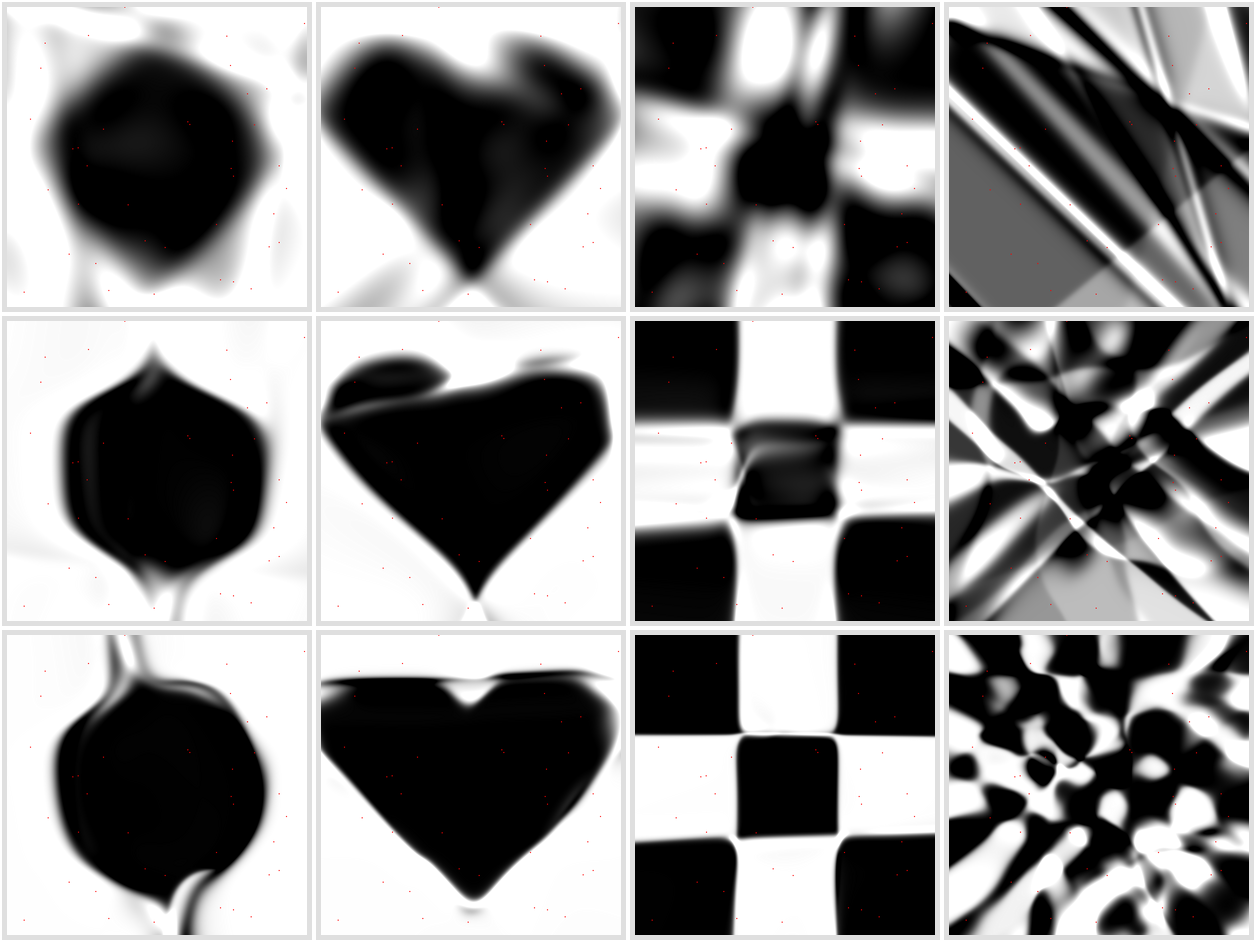
\includegraphics[width=0.9\textwidth]{data/frame00900.png}}

\begin{uloha}
Pozri si \link{\rootpath/evolution.mp4}{video} z predchádzajúceho experimentu. Čo sa z neho dá vidieť? 
Naprogramuj podobný experiment.  
Ako by sa dalo trénovanie urýchliť lepšou voľbou parametrov (veľkosť siete, veľkosť vzorky, dĺžka 
  epochy)?
\end{uloha}

\section*{Projekt: rozpoznávanie písaných číslic}
\label{projekt.cislice}
\setlength{\fboxsep}{0pt}%
\setlength{\fboxrule}{0.2pt}%

Výsledkom tohoto projektu bude program, v ktorom môžeš myšou nakresliť číslicu, program ju rozpozná a zasvieti príslušné číslo. Vyzerať by to
malo nejak takto\footnote{Výsledný program si môžeš vyskúšať tu: \href{https://beda.dcs.fmph.uniba.sk/mnist/digits.html}{\nolinkurl{https://beda.dcs.fmph.uniba.sk/mnist/digits.html}}}:

\vskip 2ex
\centerline{
  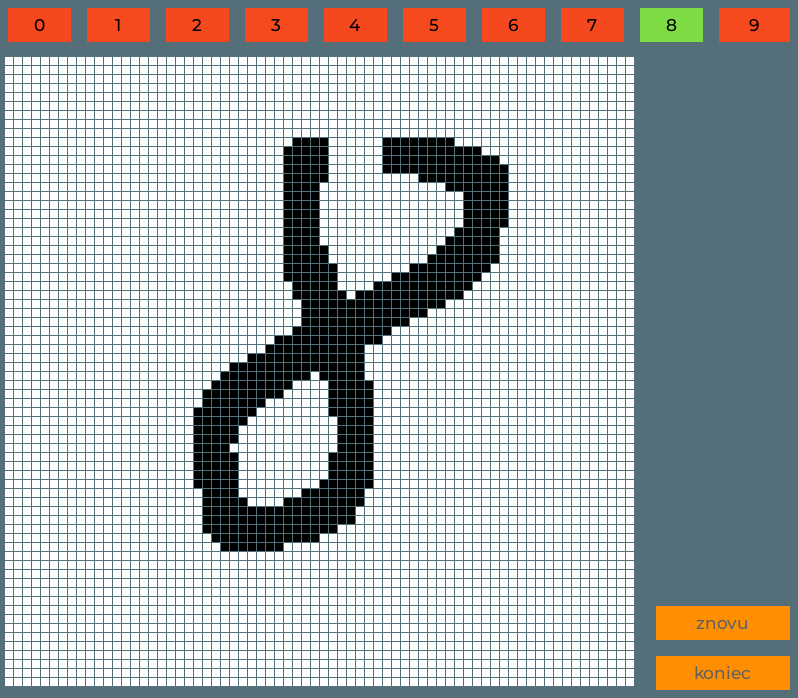
\includegraphics[width=0.45\textwidth]{data/mnist_app.png}
%  \hfill
%  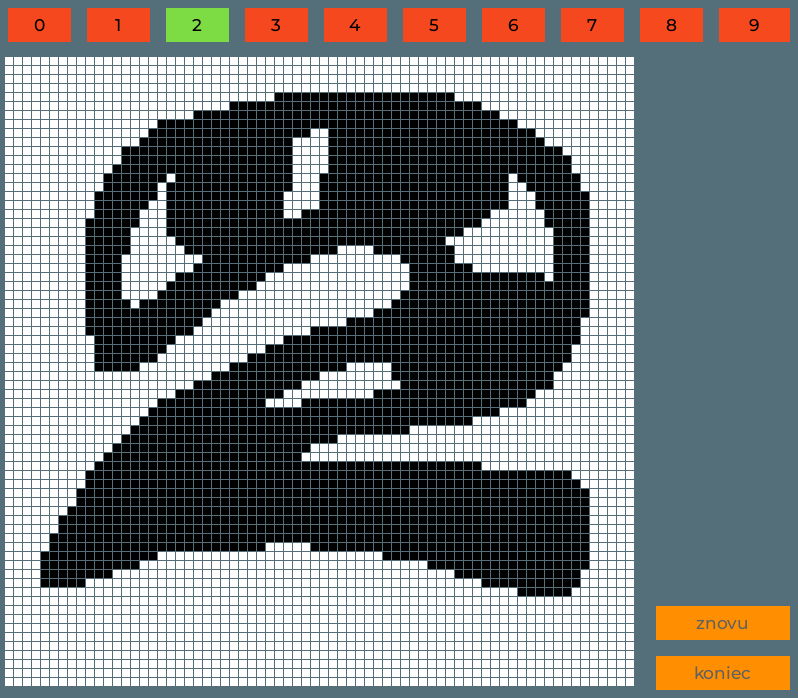
\includegraphics[width=0.45\textwidth]{data/mnist_app2.png}
}

Namiesto toho, aby som sa snažil naprogramovať tvary jednotlivých číslic, natrénujem na rozpoznávanie neurónovú sieť: každý pixel zo vstupu bude jeden vstupný neurón s hodnotou od
$-1$ pre 
bielu po $1$ pre čiernu. Na 
výstupnej vrstve bude 10 neurónov a každý bude reprezentovať jednu číslicu (čím väčšia hodnota neurónu, tým viac si sieť myslí, že je na vstupe daná číslica).
Aby som sieť mohol trénovať, potrebujem veľa príkladov napísaných číslic. Americký NIST (National Institute of Standards and Technology) má verejnú
\link{https://www.nist.gov/srd/nist-special-database-19}{databázu} rukou písaných písmen a číslic, ktorá sa dá použiť. Tá časť, čo ma zaujíma, sú rukou písané číslice,
každá je čierno-biely obrázok rozmerov $128\times128$ vo formáte png, napr:

\fbox{
\includegraphics[width=2cm]{data/mnist_2.png}}
\hfill
\fbox{
\includegraphics[width=2cm]{data/mnist_8.png}}
\hfill
\fbox{
\includegraphics[width=2cm]{data/mnist_2b.png}}
\hfill
\fbox{
\includegraphics[width=2cm]{data/mnist_4.png}}
\hfill
\fbox{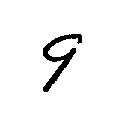
\includegraphics[width=2cm]{data/mnist_9.png}}
\hfill
\fbox{
\includegraphics[width=2cm]{data/mnist_3.png}}

\vskip 1ex
Na použitie v neurónovej sieti si ich potrebujem pripraviť. Jednak mať $128\times128=16384$ vstupných neurónov by bolo priveľa a jednak by sieť bola citlivá na posunutie. Napr.
tieto dve verzie dvojky sú takmer rovnaké, ale aktivované by boli úplne rôzne vstupné neuróny:

\vskip 2ex
\centerline{\fbox{
\includegraphics[width=4cm]{data/mnist_shift.png}}}


Povedal som si, že mi bude stačiť $26\times26=676$ vstupných neurónov. 
Predspracovanie obrázka robím takto: zistím si bounding box, t.j. najmenší obdĺžnik, v ktorom sú všetky
čierne pixely. Potom ho upravím na štvorec podľa dlhšej strany:

\vskip 2ex
\centerline{\fbox{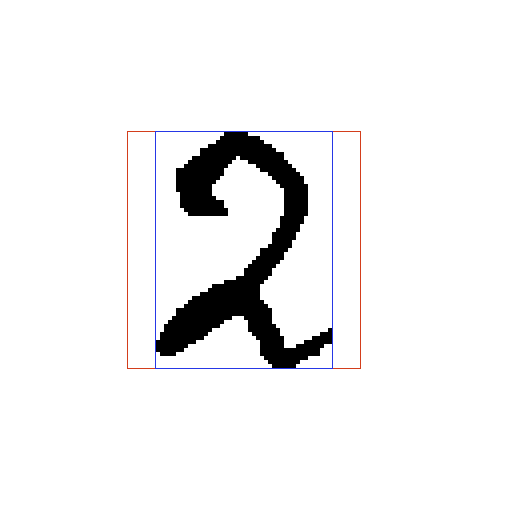
\includegraphics[width=4cm]{data/mnist_2bbox.png}}}

Štvorec vyrežem, zmenším na rozmer $18\times18$ a nájdem ťažisko čiernych (sivých) pixelov:

\vskip 3ex
\centerline{\fbox{%

\begin{tikzpicture}[scale=0.35]
  \foreach \l[count=\i] in {%
{ 255, 255, 255, 255, 255, 255, 255, 255, 255, 255, 255, 255, 255, 255, 255, 252, 251, 255 },
{ 255, 255, 255, 253, 254, 255, 255, 255, 255, 255, 255, 255, 255, 254, 252, 255, 255, 255 },
{ 255, 255, 254, 255, 255, 251, 254, 255, 255, 255, 255, 255, 253, 255, 255, 186, 128, 254 },
{ 255, 254, 255, 230, 248, 255, 255, 254, 255, 255, 255, 254, 255, 254, 99, 0, 0, 237 },
{ 251, 255, 151, 0, 40, 89, 231, 255, 254, 255, 255, 253, 255, 76, 0, 0, 99, 255 },
{ 255, 190, 0, 0, 0, 0, 150, 255, 251, 255, 251, 255, 132, 0, 3, 11, 239, 255 },
{ 255, 18, 0, 3, 71, 0, 148, 255, 251, 253, 255, 221, 13, 0, 0, 166, 255, 252 },
{ 95, 0, 20, 174, 255, 91, 155, 255, 252, 249, 255, 120, 0, 0, 94, 255, 252, 255 },
{ 0, 13, 216, 255, 251, 255, 252, 255, 252, 255, 255, 46, 0, 6, 240, 255, 247, 254 },
{ 56, 0, 185, 255, 249, 253, 255, 249, 255, 251, 73, 0, 0, 0, 85, 206, 255, 255 },
{ 177, 0, 35, 250, 255, 250, 255, 255, 240, 45, 0, 99, 156, 6, 0, 14, 93, 223 },
{ 255, 73, 0, 86, 255, 255, 248, 153, 21, 0, 155, 255, 255, 215, 150, 12, 0, 33 },
{ 255, 245, 79, 0, 36, 60, 15, 0, 42, 207, 255, 253, 250, 255, 255, 246, 99, 0 },
{ 253, 255, 255, 99, 2, 0, 42, 173, 255, 255, 250, 255, 255, 252, 250, 255, 34, 125 },
{ 255, 253, 255, 255, 237, 233, 255, 255, 254, 252, 255, 255, 255, 251, 255, 148, 0, 246 },
{ 255, 255, 254, 252, 255, 255, 255, 251, 254, 255, 255, 255, 254, 255, 255, 72, 184, 255 },
{ 255, 255, 255, 255, 253, 253, 254, 255, 255, 255, 255, 255, 255, 255, 252, 253, 255, 254 },
{ 255, 255, 255, 255, 255, 255, 255, 255, 255, 255, 255, 255, 255, 255, 255, 255, 253, 255 }} {
    \foreach \v[count=\j] in \l {
      \fill[fill={rgb,255:red,\v; green,\v; blue,\v}] (\i,-\j) rectangle ++(0.9,0.9);
    }
  }

  \fill[red](8,-8) rectangle ++(0.9,0.9);
\end{tikzpicture}}}

Napokon výsledok vycentrujem tak, aby ťažisko bolo v strede štvorca $26\times26$.
Týmto spôsobom dostanem všetky číslice rovnako veľké a rovnako umiestnené. Ak budem tým 
istým spôsobom spracovávať aj nakreslené vzory v programe, nebudem mať problémy s rôzne veľkými a 
rôzne posunutými číslami. Výsledok spracovania niektorých čísel z trénovacieho datasetu vyzerá  takto (všimni si drobné
rozdiely v typickom písaní niektorých číslic oproti Slovensku):


\vskip 2ex
\centerline{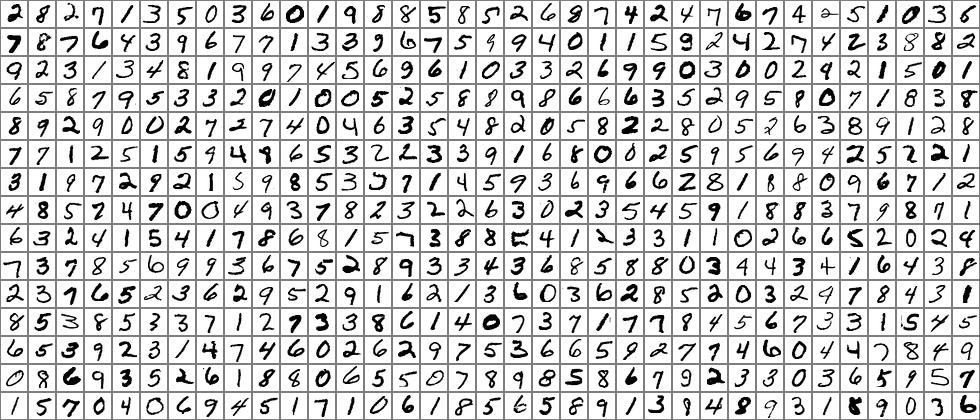
\includegraphics[width=\textwidth]{data/mnist.png}}

Vieme, čo chceme dosiahnuť, tak to môžeme začať programovať. Najprv si spravím pomocné triedy pre pixel a obdĺžnik

\vbox{\begin{lstlisting}
struct Point {
  int _p[2];
  Point &operator=(const Point &a);
  int &x() { return _p[0]; }
  int &y() { return _p[1]; }
  int x() const { return _p[0]; }
  int y() const { return _p[1]; }
  int &operator[](int i) { return _p[i]; }
  int operator[](int i) const { return _p[i]; }
  Point &operator+=(const Point &p);
  Point &operator*=(double a);
};
\end{lstlisting}}

\vbox{\begin{lstlisting}
struct Box {
  Point p[2];   // ľavý horný a pravý dolný okraj
  Point &operator[](int i) { return p[i]; }
  Point operator[](int i) const { return p[i]; }
  int x() const { return p[1].x() - p[0].x(); }
  int y() const { return p[1].y() - p[0].y(); }
  Box &expand(const Point &q); // rozšír obdĺžnik tak, aby obsahoval bod q
  Point center() const;
};
\end{lstlisting}}

Doprogramovať zvyšné metódy by malo byť priamočiare. Ďalej si urobím pomocnú triedu na uloženie
štvorcového obrázka rozmerov $d\times d$:

\vskip 2ex
\vbox{\begin{lstlisting}
using u8 = uint8_t;

struct Bytes {
  std::vector<u8> a;
  int d, n;
  u8 sentinel;
  Bytes(int _d) : d{_d}, n{d * d} { 
    a.resize(n, 255); // miesto na štvorec d x d, celý biely
  }
  u8 &operator()(int x, int y);
  u8 operator()(int x, int y) const;
  Point pos(int i) const { 
    return Point{i % d, i / d}; // súradnice i-teho pixelu
  }
  Point cog() const; // ťažisko
  Box bbox() const;  // bounding box
};
\end{lstlisting}}

Premennú \vb{sentinel} som použil na to, aby som mohol kontrolovať, či parametre v \vb{operator()}
nie sú mimo rozsahu. Keďže vraciam referenciu, potrebujem vrátiť niečo, kam sa dá beztrestne zapisovať.

\vskip 2ex
\vbox{\begin{lstlisting}
u8 &Bytes::operator()(int x, int y) {
  if (x < 0 || y < 0 || x >= d || y >= d) return sentinel;
  return a[x + y * d];
}
\end{lstlisting}}

Nájsť bounding box je jednoduché

\vskip 2ex
\vbox{\begin{lstlisting}
Box Bytes::bbox() const {
  Box b{Point{n, n}, Point{0, 0}};
  for (int i = 0; i < n; i++)
    if (a[i] < 255) b.expand(pos(i));
  return b;
}
\end{lstlisting}}

Ďalej budem potrebovať výrez naškálovať na rozmer $18\times18$. Aj keď sa to nezdá, škálovanie je celkom zložitý problém, ak ho chceš spraviť poriadne. Ak by som 
chcel iba napr. zmenšiť obrázok na polovicu, tak jednému pixelu výsledného obrázka prislúchajú štyri pixely (štovrec $2\times2$) z pôvodného. Stačí mi preto spraviť
priemer z tých štyroch a je to. Ak ale rozmer nového ovrázka nie je deliteľom pôvodného, začnú problémy. Pre naše účely to nie je zase také dôležité, ale rozhodol som sa
spraviť výnimku a použiť externú knižnicu, konkrétne škálovaciu knižnicu 
\link{https://github.com/avaneev/avir}{Avir}. Používa sa ľahko. Keďže všetko v nej je šablóna, stačí nakopírovať súbor
\link{https://github.com/avaneev/avir/raw/master/avir.h}{avir.h} do pracovného adresára a použiť \prg~#include "avir.h"~.
Potom môžeš vyrobiť premennú typu\footnote{\indexItem{Prg}{šablóny s default parametrami}tie prázdne zátvorky \prg~<>~ znamenajú, že \prg~CImageResizer~ je šablóna s default parametrom, podobne, ako keď majú
default parametre funkcie. Konkrétne \prg~avir::CImageResizer<>~ je to isté ako \prg~avir::CImageResizer< avir::fpclass_def<float> >~} \prg~avir::CImageResizer<>~. Konštruktor dostane ako parameter počet bitov na farbu, v našom prípade $8$.
Celú prácu potom urobí metóda \prg~resizeImage~

\vskip 2ex
\vbox{\begin{lstlisting}
avir::CImageResizer<>::resizeImage(
    const u8 *src,                     // pointer na dáta pôvodného obrázka
    const int src_w, consit int src_h, // rozmery pôvodného obrázka
    int lineSize,                      // veľkosť riadka, môže vždy ostať 0
    u8 *dst,                           // pointer na dáta výsledného obrázka
    const int dst_w, const int dst_h,  // výsledné rozmery
    const int numChan,                 // počet kanálov na pixel, pre nás 1 
                                       // (napr. pre RGB by bolo 3, pre RGBA 4)
    const double k                     // krok algoritmu, tu vždy môže ostať 0
  );
\end{lstlisting}}

Posledná vec, ktorú potrebujem, je nájsť ťažisko. To spravím tak, že zrátam vážený priemer pixelov (biely má váhu 0, čierny váhu 255):

\vskip 2ex
\vbox{\begin{lstlisting}
Point Bytes::cog() const {
  Point p{0, 0};
  int s = 0;
  for (int i = 0; i < d * d; i++) {
    u8 v = 255 - a[i];
    Point q = v * pos(i);
    s += v;
    p += q;
  }
  for (int i = 0; i < 2; i++) 
    p[i] = (int)((double)(p[i]) / (double)s);
  return p;
}
\end{lstlisting}}

Celá funkcia na spracovanie obrázku vyzerá takto:

\vskip 2ex
\vbox{\begin{lstlisting}
void processImage(Bytes &in, Bytes &out) {
  Box bb = in.bbox();
  int d = 1 + max(bb.x(), bb.y());  // dlhšia strana bounding boxu

  // o je ľavý horný pixel vyrezaného štvorca
  Point o{bb[0].x() - (d - bb.x()) / 2, bb[0].y() - (d - bb.y()) / 2};
  Bytes crop(d);  // sem uložím vyrezaný štvorec d x d
  int t = 0;
  for (int i = 0; i < d; i++)
    for (int j = 0; j < d; j++) {
      in.sentinel = 255;  // ak som mimo rozsahu, prečítam bielu
      crop.a[t++] = in(o.x() + j, o.y() + i);
    }

  Bytes rsz(sc); // sem uložím naškálovaný výsledok
  imageResizer.resizeImage(crop.a.data(), d, d, 0, rsz.a.data(), sc, sc, 1, 0);

  Point c = rsz.cog(); // ťažisko
  o = Point{dim / 2 - c.x(), dim / 2 - c.y() - 1}; // okraj vycentrovaného štvorca

  for (int i = 0; i < sc; i++)
    for (int j = 0; j < sc; j++)
        out(o.x() + j, o.y() + i) = rsz(j, i);
}

\end{lstlisting}}

Takto som spracoval celý dataset. Výsledok je v súbore
\link{\rootpath/mnist.zip}{mnist.zip} kde je pre každú číslicu jeden dlhý binárny súbor. V ňom je najprv počet obrázkov ako 32-bitový integer a za ním
idú jednotlivé $26\times26$ obrázky za sebou jeden byte na každý pixel, takže
prečítať to viem takto:

\vskip 2ex
\vbox{\begin{lstlisting}
vector<vector<Bytes>> dataset(10); // pre každú číslicu je zoznam obrázkov

for (int num = 0; num < 10; num++) {
  stringstream ss;
  ss << "./mnist/" << num << ".bin";
  ifstream f(ss.str(), ios::binary);
  uint32_t x;
  f.read((char *)&x, 4);  // prečítam 32 bitov (4 byty) počet obrázkov
  while (x-- > 0) dataset[num].emplace_back(dim); // vyrobím miesto pre obrázky
  for (auto &d : dataset[num]) 
      f.read((char *)(d.a.data()),  dim * dim);   // postupne všetky prečítam
}
\end{lstlisting}}

\begin{uloha}
  Natrénuj neurónovú sieť na datasete číslic. Do triedy \vb{Network} pridaj metódy \vb{save} a \vb{load} a natrénovanú sieť ulož do súboru.
\end{uloha}

Ja som použil sieť s vrstvami so \vb{676,300,100,10} neurónmi a trénoval som po epochách 1000 iterácií vždy na vzorke 200 náhodne vybratých číslic.

\vskip 4ex
Keď už je natrénovaná sieť uložená v súbore, ostáva spraviť program, ktorý ju používa a v ktorom sa
dajú kresliť číslice. Na to sa dajú použiť widgety z kapitoly~\ref{sect:dedicnost}. 
Hlavné okno bude \vb{VLayout mainWindow}, v ktorom budú dva \vb{HLayout}y: \vb{topBar}
a \vb{mainArea}. V \vb{topBar}
desať widgetov typu \vb{Bulb}, ktoré zobrazujú jednotlivé číslice. V \vb{mainArea}
bude vľavo widget typu \vb{Canvas}, ktorý sa stará o kreslenie a vpravo \vb{VLayout buttonArea} 
s gombíkmi:

\vskip 2ex
\vbox{\begin{lstlisting}
Canvas *canvas = nullptr;
Bulb *bulbs[10];
...

int main() {
  ...
  VLayout mainWindow;
  canvas = new Canvas();
  auto topBar = new HLayout();
  topBar->fixedHeight = 52;
  auto mainArea = new HLayout();
  auto buttonArea = new VLayout();
  buttonArea->fixedWidth = 150;
  Button *quitButton = new Button("koniec");
  Button *clearButton = new Button("znovu");

  for (int i = 0; i < 10; i++) {
    bulbs[i] = new Bulb(to_string(i));
    (*topBar) << bulbs[i];
  }

  mainWindow << topBar << mainArea;
  (*mainArea) << canvas << buttonArea;
  (*buttonArea) << new Widget() << clearButton << quitButton;

  ...
}
\end{lstlisting}}

Widget \vb{Bulb} môžeme spraviť modifikáciou \vb{Button}: bude vždy disabled, aby sa naňho
nedalo klikať. Navyše bude mať metódu \vb{set(double d)}, ktorá nastaví pozadie od
červenej po zelenú. Na to môžem použiť \vb{Gradient} z úlohy~\ref{uloha:gradient}.

\vskip 2ex
\vbox{\begin{lstlisting}
struct Bulb : Button {
  static const Gradient g;
  Bulb(const std::string &_txt) ;
  void set(double val) ;
};

const Gradient Bulb::g("gradient.gpf");
\end{lstlisting}}

Nakoniec treba dorobiť triedu \vb{Canvas}. V nej budem mať \vb{Bytes img} pre obrázok 
(napr. $70\times70$), v metóde i\hbox{\vb{render}} ho vykreslím zo štvorčekov. Zároveň budem
v metódach \vb{onMouseDown} a \vb{onMouseUp} sledovať polohu myši a kresliť. Keďže
myš sa môže pohybovať dosť rýchlo, je lepšie vždy vykresliť čiaru od posledného zapamätaného
miesta po súčasné. Na to môžem použiť algoritmus kreslenia čiary z úlohy~\ref{uloha:editor}.

\vskip 2ex
%\vbox{
\begin{lstlisting}
struct Canvas : Widget {
  const int dim = 70;
  int pxdim, spacing;  // rozmer štvorčeka a medzeru medzi nimi
                       // si budem nastavovať v resize
  Bytes img;
  bool painting;       // či je stlačený gombík myši
  SDL_Point lastMouse; // posledná poloha myši, odtiaľ kreslím čiaru

  Canvas();             // konštruktor
  ~Canvas();

  void clear();
  void line(SDL_Point,SDL_Point); // vykresli čiaru
  void resize(SDL_Rect scr);      // nastaví všetko potrebné pri zmene okna
  void render(SDL_Renderer *renderer);

  void onMouseDown(SDL_MouseButtonEvent& e);
  void onMouseUp(SDL_MouseButtonEvent& e);

  ... // pomocné metódy
};
\end{lstlisting}
%}

V hlavnom programe v pravidelných intervaloch spustím sieť na aktuálnom vstupe:

\vskip 2ex
\vbox{\begin{lstlisting}
void run_net() {
  auto &inp = canvas->img;     // nakreslený obrázok
  Matrix in(dim * dim, 1);     // vstup pre sieť

  Bytes tmp(inp.d);            // pred zmenšením  vstup 
                               // trochu rozmažem
  int d = inp.d;
  inp.sentinel = 255;
  for (int i = 0; i < d; i++)
    for (int j = 0; j < d; j++) {
      int v = 0;
      for (int di : {-1, 0, 1})
        for (int dj : {-1, 0, 1}) v += inp(i + di, j + dj);
      tmp(i, j) = u8(v / 9);
    }

  Bytes img(26);
  processImage(tmp, img);      // zmenši a vycentruj

  // vyrob vstup pre sieť a spusti ju
  for (int i = 0; i < 26 * 26; i++)
    in(i, 0) = 1.0 - 2.0 * (double)img.a[i] / 255.0;
  auto &out = net.feed(res.in);

  // nastav farby podľa výsledku
  for (int i = 0; i < 10; i++) bulbs[i]->set(tanh(out(i, 0)));
}
\end{lstlisting}}

\begin{uloha}
  Naprogramuj GUI tak, aby zyeralo ako screenshot na začiatku kapitoly.
\end{uloha}

\newpage
\phantom{aa}
\vfill
... a to je nateraz všetko. Je veľmi veľa vecí, ktoré sme tu nespomenuli, ale ako 
stručná odpoveď na otázku \cmd{``Ako sa programuje v C++?''} to snáď stačí.

\centerline{\usymH{1F514}{2.5cm}}

